\section{Fundamentals}

\subsection{Microstates and Macrostates}

A specific microscopic configuration of a system is called a microstate. The more loose term is macrostate which specifies the general or macroscopic properties of a system. In the coin-flipping experiment, a microstate contains the state of each coin and a macrostate is the number of heads or tails.

\begin{figure}[H]
	\centering
	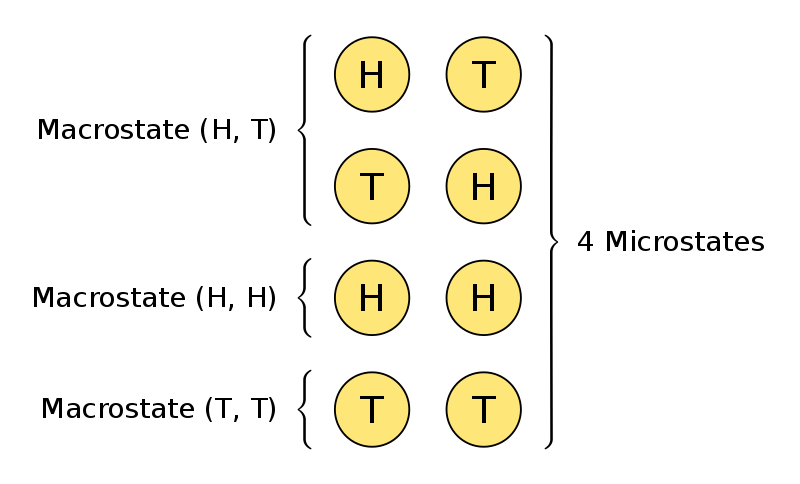
\includegraphics[width=120mm]{5.png}
	\caption{Microstate and macrostate of the experiment involving two coin flips}
\end{figure}

Each macrostate has some number of microstates and it is called multiplicity, denoted by $\Omega$. For the image above, $\Omega(\text{0 heads})=1$, $\Omega(\text{1 heads})=2$, $\Omega(\text{2 heads})=1$. The total number of microstates is $\Omega(\text{all})=1+2+1=4$. The probability of getting $n$ heads is $\frac{\Omega(n)}{\Omega(\text{all})}$. \\

Macroscopic state: description of a system based on macroscopic observables only (not microscopic, atom-by-atom ones). E.g. total energy vs the distribution of energy. Other examples include temperature, volume and pressure.

\begin{texample}
	You have $13$ cards, $6$ red ($R$) and $7$ black ($B$). You shuffle them and place them face up in two rows. The top row has $5$ cards, the bottom row $8$. If you do this many times, what number of red cards will the top row have most often? \\
	
	The total number of arrangements is $\Omega(\text{all})=\frac{13!}{6!7!}=1716$. \\
	
	To determine the most likely number of red cards, we count the number of arrangements when the top row has $0, 1, 2, 3, 4, 5$ red cards. For example, to count the number of arrangements for the top row with $2$ red cards, $\binom{5}{2}=\frac{5!}{2!3!}=10$. To get the total number of arrangements we multiply the results, for example, the total number of arrangements with $3$ red cards at the top is $10(56)=560$. After that, we calculate probabilities and compare. \\
	
	Let $n_T$ and $n_B$ denote the number of red cards at the top and bottom rows respectively. Let $\Omega_T$ denote the number of arrangements for the top row created with $n_T$ red cards, same for $\Omega_B$. $\Omega_{TB}=\Omega_T\Omega_B$ is the total number of arrangements.
	
	\begin{center}
		\begin{tabular}{l|l|l|l|l|l|l}
			$n_T$ & 0 & 1 & 2 & 3 & 4 & 5 \\
			\hline
			$\Omega_T$ & 1 & 5 & 10 & 10 & 5 & 1 \\
			\hline
			$n_B$ & 6 & 5 & 4 & 3 & 2 & 1 \\
			\hline
			$\Omega_B$ & 28 & 56 & 70 & 56 & 28 & 8 \\
			\hline
			$\Omega_{TB}$ & 28 & 280 & 700 & 560 & 140 & 8 \\
			\hline
			$\frac{\Omega_{TB}}{\Omega(\text{all})}$ & 0.016 & 0.163 & 0.408 & 0.326 & 0.082 & 0.005
		\end{tabular}
	\end{center}
	
	From the table, we see that the top row will most likely have $2$ red cards. \\
	
	Also notice that $28+280+700+560+140+8=1716$. \\
	
	If we were to compute the average number of red cards in the top row, we use the following relation: $\sum_{n=0}^5 nP_n$ where $P_n$ is the probability of getting $n$ red cards in the top row. This gives:
	
	$$0(0.016) + 1(0.163) + 2(0.408) + 3(0.326) + 4(0.082) + 5(0.005)=2.31$$
	
	This playing card example has applications in statistical mechanics for modelling two-state systems which we will see later.
\end{texample}

\subsection{Thermal Equilibrium and Zeroth Law of Thermodynamics}

The basic fact of thermodynamics is when objects of different temperature contact each other, heat flows from the warmer object to the colder object. The colder object warms up until thermal equilibrium is reached. This transfer of energy is an irreversible process. \\

Recall that heat is a spontaneous flow of energy on a microscopic scale. ``warmer'' means to be able to give more heat and ``colder'' means to be able to give off less heat. Temperature is the measure of the ability to give off heat. \\

Zeroth law of thermodynamics states that if two objects A and B are immediately in thermal equilibrium when brought together, and A and C are immediately in thermal equilibrium when brought together, then B and C are also in thermal equilibrium. \\

Thermal equilibrium is a state that any two objects will reach if they are in thermal contact (able to exchange heat) long enough. They might have different energy but have the same temperature. Being in equilibrium means things are not changing macroscopically. A thermometer is a system that allows us to visualize equilibrium. \\

A heat bath or reservoir is a system large enough s.t. the temperature is essentially unchanged after supplying or absorbing energy with much smaller systems. \\

\begin{texample}
	You have a standard deck of $52$ cards which consists of $26$ red cards and $26$ black cards. The deck is shuffled well, what is the probability that the first five cards contain $3$ red cards and $2$ black cards? What is the probability if the deck is large enough? \\
	
	We count the number of ways to draw $3$ red cards from the set of $26$ red cards: $\binom{26}{3}$ and the number of ways to draw $2$ black cards from the set of $26$ black cards: $\binom{26}{2}$. Then multiply the result and divide it by the number of ways to draw $5$ cards from the deck: $\binom{52}{5}$. This gives $P(3R,2B)=\frac{\binom{26}{3}\binom{26}{2}}{\binom{52}{5}}$. \\
	
	Alternative approach: Count the number of combinations of a $5$ card hand that contains $3$ red and $2$ black: $\binom{5}{3}$. Then count the number of ways to rearrange the remaining cards in the deck: $\binom{52-5}{26-3}$. Finally count the number of ways to arrange the deck: $\binom{52}{26}$. This gives $P(3R,2B)=\frac{\binom{5}{3}\binom{52-5}{26-3}}{\binom{52}{26}}$. \\
	
	To approximate the probability when the deck is large, we rewrite things a bit:
	
	\begin{align*}
		P(3R,2B)&=\frac{\binom{26}{3}\binom{26}{2}}{\binom{52}{5}} \\
		&=\frac{\frac{26!}{3!23!}\frac{26!}{2!24!}}{\frac{52!}{5!47!}} \\
		&=\frac{5!}{3!2!}\frac{\frac{47!}{23!24!}}{\frac{52!}{26!26!}} \\
		&=\frac{5!}{3!2!}\frac{(52-5)!26!26!}{52!(26-3)!(26-2)!} \\
		&=\frac{5!}{3!2!}\frac{26(26-1)(26-2)26(26-1)}{52(52-1)(52-2)(52-3)(52-4)} \\
		&\approx \frac{5!}{3!2!}\frac{26^5}{56^5} \\
		&\approx \frac{5!}{3!2!}\frac{1}{2^5}
	\end{align*}
	
	We conclude that the suitable approximation is $\frac{\binom{5}{3}}{2^5}$. This gets better when the deck is larger. \\
	
	This example illustrates the concept of heat bath. The larger the deck is, taking out a few cards will have almost no effect on the probability.
\end{texample}

As a demonstration of the thermodynamic process, consider two coupled lattices of oscillators where each particle has either $0$ or $1$ quanta of energy.

\begin{figure}[H]
	\centering
	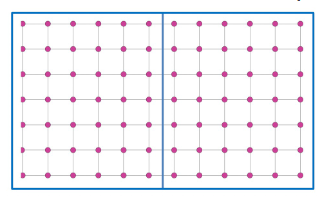
\includegraphics[width=80mm]{6.png}
	\caption{Two-state system example}
\end{figure}

The two systems can exchange energy.

\begin{texample}
	We have two systems $A$ and $B$. $A$ has $5$ particles and $B$ has $8$ particles. There are $6\epsilon$ units of energy. How many units of energy is likely in $A$? Average units of energy in $A$? \\
	
	\begin{figure}[H]
		\centering
		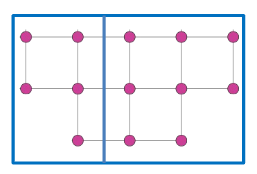
\includegraphics[width=80mm]{7.png}
		\caption{Two-state system}
	\end{figure}
	
	This is the same as the card rearrangement example we did earlier, so the answer is $2\epsilon$. The average energy units in $A$ is also $2.31\epsilon$. This is the amount of energy reached when the system reaches thermal equilibrium.
	
	\begin{figure}[H]
		\centering
		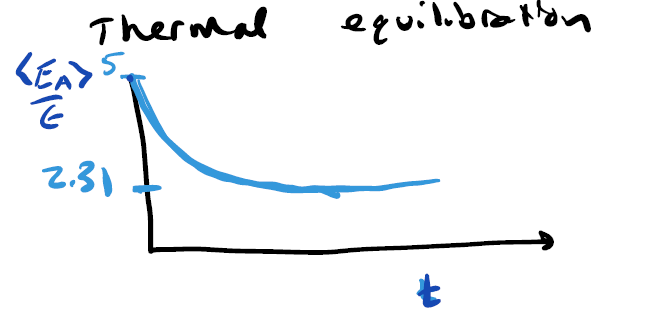
\includegraphics[width=80mm]{10.png}
		\caption{If we start with $5$ units of average energy in $A$, as time increases it will decrease to $2.31\epsilon$}
	\end{figure}
	
	This example illustrates that a system can flow its energy spontaneously (with some fluctuations) until it stops at the most likely macrostate (the one with the highest multiplicity). This is the second law of thermodynamics. \\
	
	So why we can treat thermodynamical systems as card games? It is based on the fundamental assumption in statistical mechanics: ``All microstates are equally likely'' $P(s)=\frac{1}{\Omega_{total}}$.
\end{texample}

We will now explore the probability distribution for the two-state system discussed previously.

\begin{figure}[H]
	\centering
	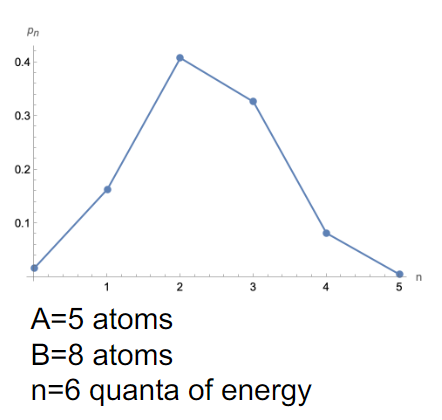
\includegraphics[width=80mm]{8.png}
	\caption{Probability distribution for the two-state system}
\end{figure}

If we increase the number of atoms and energy quantas, we get

\begin{figure}[H]
	\centering
	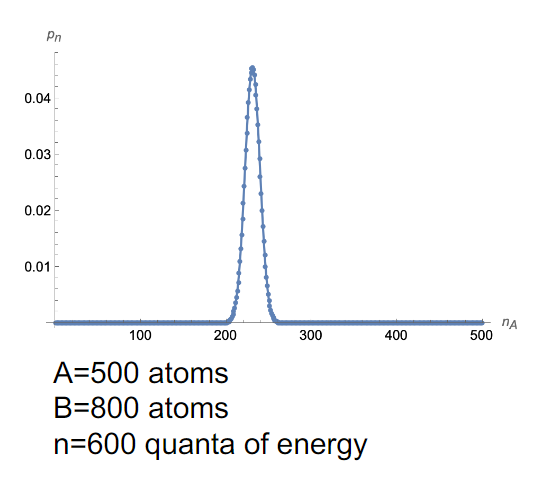
\includegraphics[width=80mm]{9.png}
	\caption{Increasing atoms and energy}
\end{figure}

The curve becomes more smooth and sharp. As the number of atoms and energy increases to infinity, the system is said to be approaching the thermodynamic limit. \\

Thermodynamic limit is when the number of components of the system is large enough so that measurable fluctuations away from the most likely macroscopic state practically never occur. \\

Fluctuations happen when there is a sudden deviation of energy from its average value. It happens often for small systems. \\

\begin{texample}
	What is the likelihood of fluctuation to pack all the possible quanta of energy to the small container for: (a) $6\epsilon$ in $(5,8)$ atoms (b) $60\epsilon$ in $(50,80)$ atoms (c) $600\epsilon$ in $(500,800)$ atoms. \\
	
	We need to find the probability for a fluctuation to pack almost all energy units into the small container. \\
	
	(a) From the previous example, we found that $P=\frac{\Omega_{TB} (5,1)}{\Omega (\text{all})}=0.005$. \\
	
	(b) $P=\frac{\Omega_{TB} (50,10)}{\Omega (\text{all})}=\frac{\binom{50}{50}\binom{80}{10}}{\binom{130}{60}}=3e-26$ \\
	
	(c) $P=\frac{\Omega_{TB} (500,100)}{\Omega (\text{all})}=\frac{\binom{500}{500}\binom{800}{100}}{\binom{1300}{600}}=3e-259$
\end{texample}

\begin{texample}
	\begin{figure}[H]
		\centering
		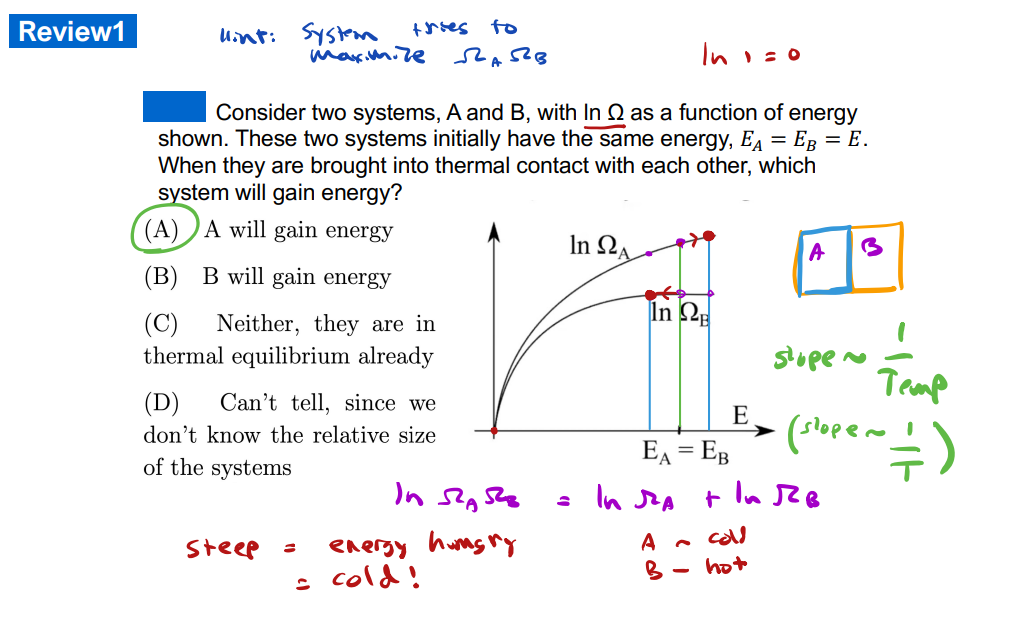
\includegraphics[width=120mm]{11.png}
	\end{figure}
	
	- $\Omega$ counts the number of microstates with associated energy, thus is a function of energy. \\
	
	- Thermal equilibrium is reached when $\Omega_A\Omega_B$ is maximized. \\
	
	- As you increase $\Omega_A$, $\Omega_B$ will decrease and vice versa (so arrows point in opposite directions). \\
	
	- The slope of $\ln\Omega$ curve will give inverse temperature $\beta$. \\
	
	- $\ln\Omega$ curves have a global maximum, so as energy increases, the curve will look like a downward parabola.
\end{texample}

To make sense of the above example, we will now derive the formula for temperature. Consider two systems $A$ and $B$ in direct thermal contact with each other, the total energy shared between systems is $E_T$. The multiplicity (number of microstates) of the $AB$ system when $A$ has energy $E_A$ and $B$ has energy $E_B=E_T-E_A$ is

$$\Omega_{AB}(E_A, E_B)=\Omega_A(E_A)\Omega_B(E_B)$$

Suppose system $A$ receives $\Delta$ units of energy from system $B$ which loses $\Delta$ units of energy in exchange, define the difference between systems to be

$$\text{diff}=\ln\Omega_{AB}(E_A+\Delta, E_B-\Delta)-\ln\Omega_{AB}(E_A, E_B)$$

We apply the logarithm identity $\ln(ab)=\ln(a)+\ln(b)$ to get

$$\text{diff}=(\ln\Omega_A(E_A+\Delta)+\ln\Omega_B(E_B-\Delta))-(\ln\Omega_A(E_A)+\ln\Omega_B(E_B))$$

$$\text{diff}=\ln\Omega_A(E_A+\Delta)-\ln\Omega_A(E_A)+\ln\Omega_B(E_B-\Delta)-\ln\Omega_B(E_B)$$

Let $f(E)=\ln\Omega(E)$ and assume $\Delta\ll E$, derivative $\frac{\partial f}{\partial E}$ at $E_0$ can be approximated as follows:

$$\left.\frac{\partial f}{\partial E}\right\vert_{E=E_0} \approx \frac{f(E_0+\Delta)-f(E_0)}{\Delta}$$

With this approximation in mind, diff becomes:

$$\text{diff}=\left.\frac{\partial \ln\Omega_A}{\partial E}\right\vert_{E=E_A}\Delta+-\left.\frac{\partial \ln\Omega_B}{\partial E}\right\vert_{E=E_B}\Delta$$

$$\text{diff}=\left(\left.\frac{\partial \ln\Omega_A}{\partial E}\right\vert_{E=E_A}-\left.\frac{\partial \ln\Omega_B}{\partial E}\right\vert_{E=E_B}\right)\Delta$$

We define a factor

$$\beta=\frac{\partial \ln\Omega}{\partial E}$$

which is porportional to inverse temperature $\frac{1}{T}$. The equation now is

$$\boxed{\text{diff}=\left(\beta_A-\beta_B\right)\Delta}$$

The physical interpretation of the system depends on the value of diff.

\begin{itemize}
	\item If $\text{diff}>0$, system $A$ gains energy which indicates $A$ is cooler. $T_A<T_B$ and $\beta_A>\beta_B$.
	\item If $\text{diff}<0$, system $A$ loses energy which indicates $A$ is warmer. $T_A>T_B$ and $\beta_A<\beta_B$.
	\item If $\text{diff}=0$, the system $AB$ is in thermal equilibrium. $T_A=T_B$ and $\beta_A=\beta_B$.
\end{itemize}

\begin{texample}
	Each table below shows the number of configurations (denoted with $\Omega$) that a system is able to reach at different energies ($E$). At each energy, all configurations available to a given system are equally likely. There are two systems, A and B. These two systems are in thermal contact with each other and share a total of $\SI{100}{\joule}$ of energy. \\
	
	\begin{center}
		\begin{tabular}{l|l}
			$E_A$ & $\Omega_A$ \\
			\hline
			$\SI{0}{\joule}$ & $1$ \\
			\hline
			$\SI{20}{\joule}$ & $10^{\num{6.92e21}}$ \\
			\hline
			$\SI{40}{\joule}$ & $10^{\num{1.32e22}}$ \\
			\hline
			$\SI{60}{\joule}$ & $10^{\num{1.86e22}}$ \\
			\hline
			$\SI{80}{\joule}$ & $10^{\num{2.26e22}}$ \\
			\hline
			$\SI{100}{\joule}$ & $10^{\num{2.52e22}}$
		\end{tabular}
		\quad
		\begin{tabular}{l|l}
			$E_B$ & $\Omega_B$ \\
			\hline
			$\SI{0}{\joule}$ & $1$ \\
			\hline
			$\SI{20}{\joule}$ & $10^{\num{6.30e21}}$ \\
			\hline
			$\SI{40}{\joule}$ & $10^{\num{1.10e22}}$ \\
			\hline
			$\SI{60}{\joule}$ & $10^{\num{1.54e22}}$ \\
			\hline
			$\SI{80}{\joule}$ & $10^{\num{1.95e22}}$ \\
			\hline
			$\SI{100}{\joule}$ & $10^{\num{2.32e22}}$
		\end{tabular}
	\end{center}
	
	(a) How much energy is in system A at thermal equilibrium? Give your answer in J. \\
	
	Thermal equilibrium happens when $\Omega_A\Omega_B$ is maximized. We will make a similar table from the cards example but since numbers are very large, we will use logarithms to turn multiplications into additions (natural base is usually used but base $10$ is for convenience).
	
	\begin{center}
		\footnotesize
		\begin{tabular}{l|l|l|l|l|l|l}
			$E_A$ & $\SI{0}{\joule}$ & $\SI{20}{\joule}$ & $\SI{40}{\joule}$ & $\SI{60}{\joule}$ & $\SI{80}{\joule}$ & $\SI{100}{\joule}$ \\
			\hline
			$\log_{10}\Omega_A$ & 0 & \num{6.92e21} & \num{1.32e22} & \num{1.86e22} & \num{2.26e22} & \num{2.52e22} \\
			\hline
			$E_B$ & $\SI{100}{\joule}$ & $\SI{80}{\joule}$ & $\SI{60}{\joule}$ & $\SI{40}{\joule}$ & $\SI{20}{\joule}$ & $\SI{0}{\joule}$ \\
			\hline
			$\log_{10}\Omega_B$ & \num{2.32e22} & \num{1.95e22} & \num{1.54e22} & \num{1.10e22} & \num{6.30e21} & 0 \\
			\hline
			$\log_{10}\Omega_{AB}$ & \num{2.32e22} & \num{2.642e22} & \num{2.86e22} & \num{2.96e22} & \num{2.89e22} & \num{2.52e22}
		\end{tabular}
	\end{center}
	
	It seems like $\Omega_A\Omega_B$ is maximized when $E_A=\SI{60}{\joule}$ and $E_B=\SI{40}{\joule}$.
	
	(b) Estimate the value of $\beta$ at thermal equilibrium (in units of $\text{J}^{-1}$). \\
	
	We can estimate $\beta$ using $\frac{\ln\Omega_2-\ln\Omega_1}{E_2-E_1}$. We choose two points in $A$ before and after equilibrium point which are $E_1=\SI{40}{\joule}$ and $E_2=\SI{80}{\joule}$. This gives
	
	$$\beta=\frac{\ln\Omega_2-\ln\Omega_1}{E_2-E_1}=\num{5.411e20}$$
\end{texample}

\subsection{Boltzmann Statistics}

\subsubsection{Boltzmann Factor}

There exists a simple formula for finding the probability to find a system in a particular microstate. Last time, we have seen that the multiplicity of a system typically increases the more energy it gets (at least up to some maximum). We focused on systems with fixed energy (microcanonical ensemble) where the fundamental assumption of statistical mechanics holds but now we will study systems with fixed $\beta$. Imagine an atom in a solid with fixed temperature $\beta$ that is in a particular quantum state (ie. having a certain amount of energy). The atom is the system of interest. We assume that each quantum state corresponds to a single microstate in this atom.

\begin{figure}[H]
	\centering
	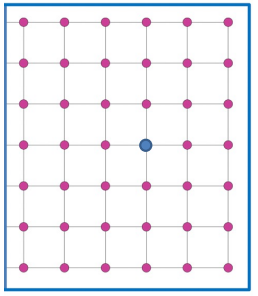
\includegraphics[width=40mm]{12.png}
	\caption{Atom in Solid}
\end{figure}

This atom is surrounded by the bath which is the rest of the solid. It is in thermal contact with the bath. The whole system (atom+bath) is isolated and this means the total energy of the whole system is constant no matter how much energy is passed back and forth between the atom and the bath. The energy that is available to the bath depends on how much energy the atom has in its quantum state. Since the atom can have many quantum states, the atom's energy is discrete while the bath's energy is continuous. \\

If the atom is isolated from the rest of the universe, it will have fixed energy. But if it interacts with lots of other atoms via bath by exchanging energy, it can change its quantum state (microstate) and some of its microstates will be more likely than others. This is because its energy is not constant since it is in thermal contact with the bath. \\

Suppose the total energy of the atom+bath system is $E_0$. Let $E$ denote the energy of the bath and $\Delta$ denote the energy of the atom which will change depending on its quantum state. By conservation of energy,

$$E+\Delta=E_0$$

The total multiplicity for the atom+bath system is (sys is atom)

$$\Omega_{tot}(E,\Delta)=\Omega_{bath}(E_0-\Delta)\Omega_{sys}(\Delta)$$

We have $\Omega_{sys}(\Delta)=1$ (the number of ways to arrange a particular microstate itself is one).

$$\Omega_{tot}(E,\Delta)=\Omega_{bath}(E_0-\Delta)$$

While it looks like the multiplicity of the bath is independent of the atom's state but not really. Depending on how much energy $\Delta$ the bath loses to the atom, $\Omega_{bath}$ will vary. To express the relationship between $\Omega_{tot}$ and $\Omega_{bath}$, we apply the first order Taylor expansion on $\ln\Omega_{tot}$ about $E_0$,

\begin{align*}
	\ln\Omega_{tot}(E,\Delta)&=\ln\Omega_{bath}(E) \\
	&=\ln\Omega_{bath}(E_0)+\left.\frac{\partial \ln\Omega_{bath}}{\partial E}\right\vert_{E=E_0}(E-E_0) \\
	&=\ln\Omega_{bath}(E_0)-\left.\frac{\partial \ln\Omega_{bath}}{\partial E}\right\vert_{E=E_0}\Delta \\
	&=\ln\Omega_{bath}(E_0)-\beta\Delta
\end{align*}

Raising $e$ to the power of both sides gives

$$\boxed{\Omega_{tot}=\Omega_{bath}(E_0)e^{-\beta\Delta}}$$

$e^{-\beta\Delta}$ is known as the Boltzmann factor.

\begin{texample}
	What is the relative likelihood of the atom having a quantum of energy $\epsilon$, vs. having no energy at all? (ie. $p(\epsilon)/p(0)$) \\
	
	$$\frac{p_\epsilon}{p_0}=\frac{\Omega_{tot}(E_0,\epsilon)}{\Omega_{tot}(E_0,0)}=\frac{\Omega_{bath}(E_0)e^{-\beta\epsilon}}{\Omega_{bath}(E_0)e^{-\beta(0)}}=e^{-\beta\epsilon}$$
	
	We got $e^{-\beta\epsilon}<1$ which indicates that the atom will most likely have zero energy.
\end{texample}

\begin{texample}
	The states of a system are labelled below, and their energies are shown (if you don't know how to read the graph, energies are macrostates, each has some number microstates. Each microstate is labelled with numbers).
	
	\begin{figure}[H]
		\centering
		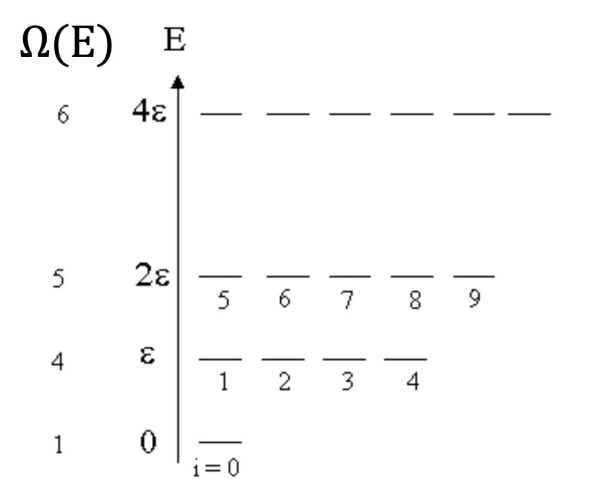
\includegraphics[width=80mm]{14.png}
	\end{figure}
	
	Find the relative likelihoods for the following pairs of microstates: (a) 2 and 4 (b) 2 and 7. \\
	
	For microstates 2 and 4, the relative likelihood is
	
	$$\frac{p_4}{p_2}=\frac{\Omega_{bath}(E_0)e^{-\beta E_4}}{\Omega_{bath}(E_0)e^{-\beta E_2}}=e^{-\beta(E_4-E_2)}=e^{-\beta(\epsilon-\epsilon)}=1$$
	
	They are equally likely. Similarly for microstates 2 and 7,
	
	$$\frac{p_7}{p_2}=e^{-\beta(E_7-E_2)}=e^{-\beta(2\epsilon-\epsilon)}=e^{-\beta\epsilon}<1$$
	
	This means microstate 2 is more likely than microstate 7: $P_2>P_7$.
\end{texample}

\begin{texample}
	Continuing from the last example, decide whether it is true that $P(E=0)=P(E=2\epsilon)$. \\
	
	We have
	
	$$\frac{P(E=0)}{P(E=2\epsilon)}=\frac{e^{-\beta(0)}}{5e^{-\beta(2\epsilon)}}=\frac15 e^{2\beta\epsilon}$$
	
	It looks like whether $\frac15 e^{2\beta\epsilon} >1$ or $\frac15 e^{2\beta\epsilon} < 1$ depends on the value of $\beta$. The former is true for low temperatures ($\beta\to\infty$) and the system is more likely to be in the state of zero energy. For high temperatures ($\beta\to0$), the ratio becomes $\frac{1}{5}<1$ and the system is more likely to be in the state of $2\epsilon$ energy. So the answer is undecidable.
\end{texample}

\subsubsection{Partition Function}

The total probability of finding the atom in some state or other must add up to one:

$$\sum_j^{\Omega_{total}}p_j=1$$

We can use this fact to find the expression for $p_i$, the probability of finding the atom in a particular microstate state $i$. We start with the relative probability expression we derived from the previous section:

$$\frac{p_j}{p_i}=e^{-\beta(E_j-E_i)}$$
$$\frac{1}{p_i} \underbrace{\left( \sum_j p_j \right)}_{=1} = e^{\beta E_i}\left( \sum_j e^{-\beta E_j} \right)$$

Rearranging the terms, we get

$$\boxed{p_i=\frac{e^{-\beta E_i}}{\sum_j e^{-\beta E_j}}=\frac{e^{-\beta E_i}}{Z(\beta)}}$$

The $Z(\beta)$ is called the partition function and it represents the sum of all state's Boltzmann factors. It depends on temperature only. From this formula, we see that the microstates with the same energy will still have the same probability.

\begin{texample}
	What is the partition function for this system?
	
	\begin{figure}[H]
		\centering
		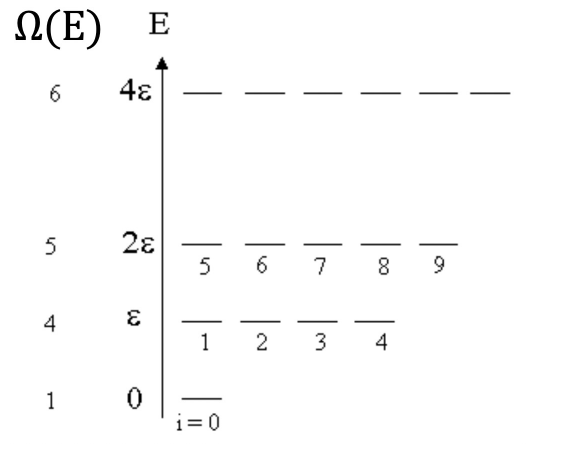
\includegraphics[width=80mm]{15.png}
	\end{figure}
	
	We have
	
	$$Z=\sum_j e^{-\beta E_j}=1+4e^{-\beta\epsilon}+5e^{-2\beta\epsilon}+6e^{-4\beta\epsilon}=\sum_E \Omega(E)e^{-\beta E}$$
\end{texample}

From the previous example, we can deduce that the probability of the system having an energy $E$ (particular macrostate) is

$$P(E)=\frac{\Omega(E)e^{-\beta E}}{\sum_E \Omega(E)e^{-\beta E}}=\frac{\Omega(E)e^{-\beta E}}{Z(\beta)}$$

\begin{texample}
	A cup of water is in a large room at temperature. Is it more likely that the cup is in a particular state
	containing zero quanta of energy than it is in a particular state with the average number of quanta of energy? \\
	
	The particular state here means a particular microstate. \\
	
	The answer is yes because if we look at this formula we derived earlier $p_i=\frac{e^{-\beta E_i}}{Z(\beta)}$, $p_i$ is largest if $E_i$ is zero.
	
	\begin{figure}[H]
		\centering
		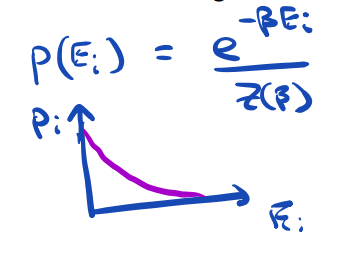
\includegraphics[width=80mm]{16.png}
		\caption{Graph of $p_i$}
	\end{figure}
	
	As a side note, even though the cup is more likely to be in the state of zero energy, its energy in thermal equilibrium is nonzero. Take a look at the following graph
	
	\begin{figure}[H]
		\centering
		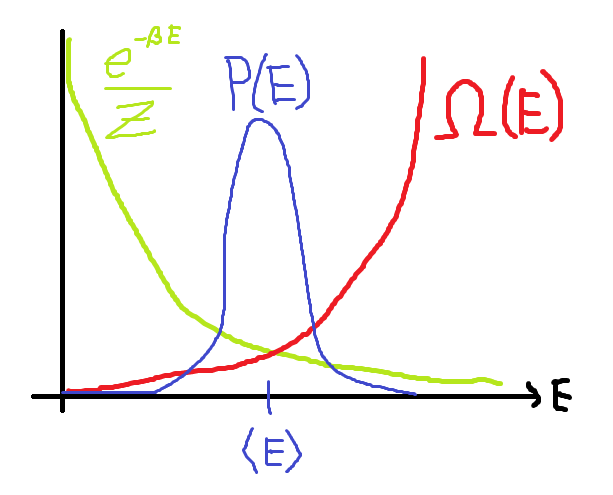
\includegraphics[width=100mm]{17.png}
		\caption{Graph of $p_i$, $\Omega$ and $P(E)$}
	\end{figure}
	
	The green line represents $p_i=\frac{e^{-\beta E_i}}{Z(\beta)}$, the red line represents number of microstates with energy $E$: $\Omega(E)$ and the blue line represents the product of the green and red lines:
	
	$$P(E)=\frac{\Omega(E)e^{-\beta E}}{Z(\beta)}$$
	
	It is averaged at $\langle E \rangle$.
\end{texample}

\begin{texample}
	A particle has $3$ possible states: $\SI{0}{\electronvolt}$, $\SI{2}{\electronvolt}$ and $\SI{3}{\electronvolt}$. If this particle is interacting with a large object with $\beta=\SI{0.5}{\per\electronvolt}$, what is its average energy? \\
	
	We have
	
	$$Z=\sum_E \Omega(E)e^{-\beta E}=e^{-0.5 (0)}+e^{-0.5 (2)}+e^{-0.5 (3)}=1.59$$
	
	The probabilities are $P(0)=\frac{1}{1.59}$, $P(2)=\frac{e^{-1}}{1.59}$, $P(3)=\frac{e^{-1.5}}{1.59}$. \\
	
	The average energy is therefore
	
	$$\langle E \rangle = \sum_i E_i P(E_i) = \SI{0}{\electronvolt}\frac{1}{1.59}+\SI{2}{\electronvolt}\frac{e^{-1}}{1.59}+\SI{3}{\electronvolt}\frac{e^{-1.5}}{1.59}=\SI{0.88}{\electronvolt}$$
\end{texample}

\begin{texample}
	A system described by the energy diagram below is in thermal equilibrium with a heat bath at temperature $T$.
	
	\begin{figure}[H]
		\centering
		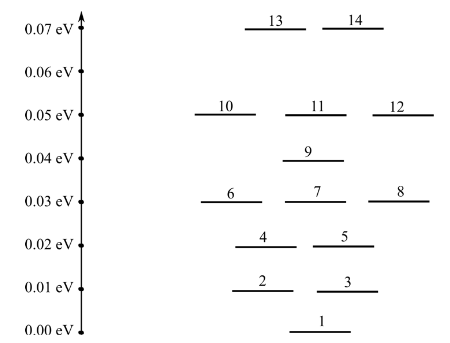
\includegraphics[width=100mm]{28.png}
	\end{figure}
	
	(a) What is the most likely energy when $T$ is very large? What if $T$ is very small? (b) Compare probabilities of $\SI{0.01}{\electronvolt}$ and $\SI{0.03}{\electronvolt}$ at high and low temperatures. (c) Finally, You have a collection of one million ($10^6$) atoms with the spectrum shown in the diagram above. The heat bath these atoms are interacting with has a very, very high temperature.  How large would you expect the fluctuations in the total energy of the one million atoms to be (make an estimate)? \\
	
	(a) The most likely energy when $T$ is large is either $\SI{0.03}{\electronvolt}$ or $\SI{0.05}{\electronvolt}$ since they both have the same number of microstates. But let's compare:
	
	\[ \frac{P(\SI{0.05}{\electronvolt})}{P(\SI{0.03}{\electronvolt})} = \frac{3e^{-\beta(0.05)}}{3e^{-\beta(0.03)}} = e^{-\beta(0.02)} < 1 \]
	
	This makes $\SI{0.03}{\electronvolt}$ more likely energy when $T$ is high. \\
	
	When $T$ is very small, $\beta$ is very large which makes $e^{-\beta E} \approx 0$. In this case, $\SI{0.00}{\electronvolt}$ is most likely since $P(\SI{0.05}{\electronvolt})\sim e^{-\beta 0.00}=1$. \\
	
	(b) We have
	
	\[ P(\SI{0.01}{\electronvolt}) \sim e^{-\beta 0.01} \]
	\[ P(\SI{0.03}{\electronvolt}) \sim 3e^{-\beta 0.03} \]
	
	The graph of these probabilities looks like the following
	
	\begin{figure}[H]
		\centering
		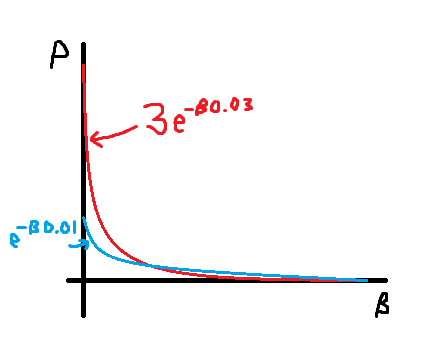
\includegraphics[width=100mm]{29.png}
	\end{figure}
	
	We see that at low temperatures (high beta), $\SI{0.01}{\electronvolt}$ is more likely than $\SI{0.03}{\electronvolt}$. \\
	
	(c) The expectation value (or average energy for a single atom) is
	
	\[ \langle E \rangle=\frac{1}{14} \left( 0.00 (1) + 0.01 (2) + 0.02 (2) + 0.03 (3) + 0.04 (1) + 0.05 (3) + 0.07 (2) \right) = \SI{0.0343}{\electronvolt} \]
	
	For the system of $N$ atoms, the total energy is $N\langle E \rangle$. The standard deviation is therefore
	
	\[ \sigma_N = \frac{N\langle E \rangle}{\sqrt{N}}=\SI{34.3}{\electronvolt} \]
	
\end{texample}

\subsubsection{Ideal Gas Kinetic Model}

In this section, we will derive the alternative form of the ideal gas law step-by-step using the statistical tools we just learned. \\

An ideal gas is a theoretical gas model made of particles that are noninteracting (have no forces between them) but interact with each other through elastic collisions, and particles have no volume exclusion (i.e. no size) but have identical mass. \\

\begin{figure}[h!]
	\centering
	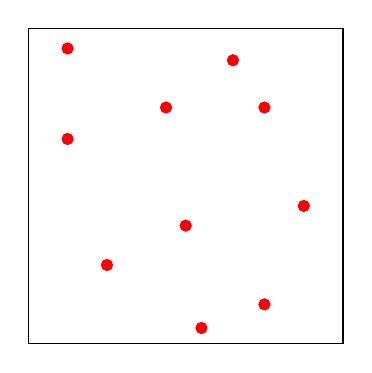
\begin{tikzpicture}
		\draw[draw = black] (0,0) rectangle (4,4);
		\draw[thick] (4,0) -- (4,4);
		\draw[fill=red, draw=red] (1,1) circle (2pt);
		\draw[fill=red, draw=red] (3,0.5) circle (2pt);
		\draw[fill=red, draw=red] (0.5,2.6) circle (2pt);
		\draw[fill=red, draw=red] (2.6,3.6) circle (2pt);
		\draw[fill=red, draw=red] (3.5,1.75) circle (2pt);
		\draw[fill=red, draw=red] (1.75,3) circle (2pt);
		\draw[fill=red, draw=red] (2,1.5) circle (2pt);
		\draw[fill=red, draw=red] (2.2, 0.2) circle (2pt);
		\draw[fill=red, draw=red] (3,3) circle (2pt);
		\draw[fill=red, draw=red] (0.5, 3.75) circle (2pt);
	\end{tikzpicture}
	\caption{Cartoon of Ideal Gas}
\end{figure}

Its properties can be summarized by the following empirical formula

$$PV=nRT$$

where $P$ is gas pressure, $V$ is container's volume, $n=N/N_A$ is number of moles in gas, $R$ is the ideal gas constant and $T$ is gas temperature. \\

We start by expressing gas pressure in terms of particles' velocity. Consider the below one-dimensional setup

\begin{center}
	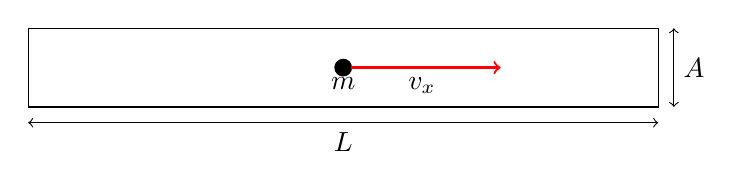
\begin{tikzpicture}[scale=4]
		\draw[draw=black] (0,0) rectangle(2,0.25);
		\filldraw (1,0.125) circle (0.75pt);
		\draw[red, ->, thick] (1.025,0.125) -- (1.5,0.125);
		\node[below] at (1,0.125) {$m$};
		\node[below] at (1.25,0.125) {$v_x$};
		\draw[<->] (0,-0.05) -- (2,-0.05);
		\draw[<->] (2.05,0) -- (2.05,0.25);
		\node[below] at (1,-0.05) {$L$};
		\node[right] at (2.05,0.125) {$A$};
	\end{tikzpicture}
\end{center}

It shows a particle of mass $m$ travelling with speed $v_x$ inside the tube of length $L$ to the right. It will hit the front wall of area $A$ and bounce back to its starting point. \\

The total time for the whole journey is

$$\Delta t = \frac{2L}{v_x}$$

The pressure applied to the wall is given by

$$P=\frac{F}{A}$$

We need to calculate the average force exerted on the wall by the particle which is given by

$$F=-\frac{\Delta p}{\Delta t}$$

(The minus sign exists because of Newton's third law.) The particle's change of momentum after it bounces off the wall is $\Delta p = -mv_x-mv_x=-2mv_x$. The force is now

$$F=\frac{-\left( -2mv_x \right)}{\frac{2L}{v_x}}=\frac{mv_x^2}{L}$$

Substituting this result into our pressure formula results in

$$P=\frac{mv_x^2}{AL}=\frac{mv_x^2}{V}$$

where $V=AL$ denotes the volume of the tube. If there are more than one particle (say $N$ particles), the pressure becomes

$$P=\sum_{i=1}^N \frac{mv_{x,i}^2}{V}$$

We can express the pressure in terms of average velocity squared $v_x^2$

$$P=\frac{Nm}{V} \left(\frac{1}{N} \sum_{i=1}^N v_{x,i}^2 \right) = \frac{Nm}{V} \langle v_x^2 \rangle$$

$$PV=Nm\langle v_x^2 \rangle$$

Next, we will express $\langle v_x^2 \rangle$ in terms of temperature. The mean-square velocity depends only on temperature, not how many particles are present to some extent. The partition function for the particle is

$$Z=\sum_{i} e^{-\beta E_i}=\sum_{i} e^{-\beta \frac{1}{2}mv_i^2}$$

Remember that index $i$ denotes possible microstates of a single particle, not each individual particle in gas. This function applies to a single particle moving in 3D space. Since each particle microstate can be expressed in terms of possible combinations of velocities $(v_x,v_y,v_z)$, we rewrite the partition function as follows

$$Z = \frac{1}{\Delta v_x \Delta v_y \Delta v_z} \sum_{v_x} \sum_{v_y} \sum_{v_z} e^{-\beta \frac{1}{2}m (v_x^2+v_y^2+v_z^2)} \Delta v_x \Delta v_y \Delta v_z$$

We add $\Delta v_x \Delta v_y \Delta v_z$ to divide the whole momentum space into little 3D cubes, since velocities are continuous quantities. $\Delta v_x \Delta v_y \Delta v_z$ can be thought of as the volume of a small portion of the momentum space. As $\Delta v_x, \Delta v_y, \Delta v_z$ gets smaller, we get the following integral

\begin{align*}
	Z&=\frac{1}{\Delta v_x \Delta v_y \Delta v_z}\int_{-\infty}^\infty\int_{-\infty}^\infty\int_{-\infty}^\infty dv_xdv_ydv_z e^{-\beta \frac{1}{2}m (v_x^2+v_y^2+v_z^2)} \\
	&=\frac{1}{\Delta v_x \Delta v_y \Delta v_z}\left[ \int_{-\infty}^\infty dv_x e^{-\beta \frac{1}{2}m v_x^2} \right]\left[ \int_{-\infty}^\infty dv_y e^{-\beta \frac{1}{2}m v_y^2} \right]\left[ \int_{-\infty}^\infty dv_z e^{-\beta \frac{1}{2}m v_z^2} \right] \\
	&=\frac{1}{\Delta v_x \Delta v_y \Delta v_z}Z_xZ_yZ_z \\
	&=\frac{1}{\Delta v_x \Delta v_y \Delta v_z}(Z_x)^3
\end{align*}

where the last line follows from symmetry. The $Z_x$ integral can be evaluated by rewriting it as a Gaussian integral

\begin{align*}
	Z_x&=\int_{-\infty}^\infty dv_x e^{-\beta \frac{1}{2}m v_x^2} \\
	&=\left( \frac{2}{\beta m} \right)^{\frac12} \underbrace{\int_{-\infty}^\infty du \: e^{-u^2}}_{\sqrt{\pi}}  = \left( \frac{2\pi}{\beta m} \right)^{\frac12}
\end{align*}

Now, the average velocity squared $\langle v_x^2 \rangle$ can be written as

$$\langle v_x^2 \rangle = \sum_i v_{x,i}^2 p_i = \frac{1}{Z}\sum_i v_{x,i}^2 e^{-\beta E_i} = \frac{1}{Z}\sum_i v_{x,i}^2 e^{-\beta \frac{1}{2}m (v_x^2+v_y^2+v_z^2)}$$

Using the similar argument as before, the average velocity squared becomes

\begin{align*}
	\langle v_x^2 \rangle &= \frac{\cancel{\Delta v_x \Delta v_y \Delta v_z}}{Z_xZ_yZ_z} \frac{1}{\cancel{\Delta v_x \Delta v_y \Delta v_z}} \int_{-\infty}^\infty\int_{-\infty}^\infty\int_{-\infty}^\infty dv_xdv_ydv_z v_x^2 e^{-\beta \frac{1}{2}m (v_x^2+v_y^2+v_z^2)} \\
	&= \frac{1}{Z_xZ_yZ_z}\left[ \int_{-\infty}^\infty dv_x v_x^2 e^{-\beta \frac{1}{2}m v_x^2} \right]\underbrace{\left[ \int_{-\infty}^\infty dv_y e^{-\beta \frac{1}{2}m v_y^2} \right]}_{Z_y} \underbrace{\left[ \int_{-\infty}^\infty dv_z e^{-\beta \frac{1}{2}m v_z^2} \right]}_{Z_z} \\
	&= \frac{1}{Z_x} \int_{-\infty}^\infty dv_x v_x^2 e^{-\beta \frac{1}{2}m v_x^2}
\end{align*}

We will use our result for $Z_x$ are rewrite this integral as another Gaussian integral

\begin{align*}
	\langle v_x^2 \rangle &= \left( \frac{\beta m}{2\pi} \right)^{\frac12} \int_{-\infty}^\infty dv_x v_x^2 e^{-\beta \frac{1}{2}m v_x^2} \\
	&= \left( \frac{\beta m}{2\pi} \right)^{\frac12} \left( \frac{2}{\beta m} \right)^{\frac32} \underbrace{\int_{-\infty}^\infty du \: u^2 e^{-u^2}}_{\frac{\sqrt{\pi}}{2}} = \frac{1}{\beta m}
\end{align*}

Substituting our average velocity squared into our ideal gas law equation gives

$$PV=Nm\langle v_x^2 \rangle=\frac{Nm}{\beta m}=\frac{N}{\beta}$$

We are almost done! Next, we will try to relate it to the empirical gas law to derive the relationship between $\beta$ and $T$

$$PV=nRT=\frac{N}{N_A}RT=\frac{N}{\beta}$$

$$\boxed{\beta=\frac{1}{k_BT}}$$

We defined the new constant $k_B=R/N_A$, known as Boltzmann constant. Substituting this result into our ideal gas law equation gives

$$\boxed{PV=Nk_BT}$$

We derived the ideal gas law in an alternate form. \\

As a corollary, we can also calculate the root mean square speed and the total kinetic energy of an ideal gas with results from this section. We showed that the mean velocity squared is

$$\langle v_x^2 \rangle=\frac{1}{\beta m}$$

Using our result for $\beta$, we get

$$\langle v_x^2 \rangle=\frac{k_BT}{m}$$

Now for each gas particle, its \textit{average} kinetic energy in the x-direction is

$$\langle E_x \rangle = \frac12m\langle v_x^2 \rangle = \frac12m\frac{k_BT}{m}=\frac12k_BT$$

Since each gas particle moves in each of the three dimensions, the overall average kinetic energy is

$$\langle E \rangle = \langle E_x \rangle + \langle E_y \rangle + \langle E_z \rangle = 3\langle E_x \rangle = \frac32k_BT$$

by symmetry. Equating this result with kinetic energy will give the formula for calculating the root mean square speed:

$$\frac12m\langle v^2 \rangle=\frac32k_BT$$

$$v_{rms}=\sqrt{\langle v^2 \rangle}=\sqrt{\frac{3k_BT}{m}}$$

or

$$v_{rms}=\sqrt{\frac{3RT}{M}}$$

where $M=m/n$ is molar mass of a gas molecule. \\

Note that the root mean square speed is not always equal to the average speed $\langle v \rangle$. It will only give an \textit{estimate} of the average speed of gas molecules. \\

Finally, for $N$ gas particles, the total thermal energy of an ideal gas is:

$$\boxed{U_{tot}=\frac32Nk_BT}$$

This should be the average thermal energy but for large $N$, fluctuations from the average will be negligible. \\

We will see the more general result of this in the later section.

\subsection{Ideal Gas Law}

As discussed in the previous section, the properties of an ideal gas is summarized by the following formula

\[ PV=nRT \]

or

\[ PV=Nk_BT \]

where $P$ is gas pressure (in pascals), $V$ is container's volume (in cubic meters), $N$ is number of molecules, $n=N/N_A$ is number of moles in gas (Avogadro's number $N_A=\SI{6.023e23}{}$), $R=\SI{8.314462}{\cubic\meter\pascal\per\kelvin\per\mole}$ is the ideal gas constant, $k_B=R/N_A=\SI{1.380649e-23}{\joule\per\kelvin}$ is Boltzmann constant, and $T$ is gas temperature (in kelvins). Sometimes pressure is measured in atmospheres ($\SI{1}{\atmosphere}=\SI{101325}{\pascal}$) and bars ($\SI{1}{\bar}=\SI{1e5}{\pascal}$) and volume is sometimes in liters ($\SI{1}{\liter}=\SI{0.001}{\cubic\meter}$). \\

It is nothing but a combination of three simple gas laws. There is Boyle's Law, which tells us that for fixed temperature $T$ and the number of gas molecules $N$, the pressure $P$ is inversely proportional to the volume $V$:

$$P \propto \frac{1}{V}$$

And there is Charles' Law, which tells us that for fixed pressure $P$ and the number of molecules $N$, the volume $V$ is directly proportional to the temperature $T$:

$$V \propto T$$

Finally,  Avogadro's Law, which tells us that for constant temperature $T$ and constant pressure $P$, The volume of gas $V$ is directly proportional to the number of molecules $N$:

$$V \propto N$$

Combining all these three laws will derive the ideal gas law shown at the beginning. \\

Also the ideal gas law is an equation of state; it depends only on the current state of the system, but not how the system got there. \\

There are numerous implications from the ideal gas law. For a given amount of gas at a given temperature, doubling the pressure squeezes the gas into exactly half as much space. Or, at a given volume, doubling the temperature causes the pressure to double.

\begin{texample}
	Consider a box of ideal gas. What happens to the gas if we (a) increase the box's volume (b) poke a hole in the box? (c) If we connect the box with another box of ideal gas with the same volume but with warmer gas, which box has more molecules? \\
	
	(a) Temperature $T$ and number of molecules $N$ are fixed (to change temperature, one must do something with molecules' average kinetic energy) but since we increased volume $V$, according to the ideal gas law $PV=Nk_B T$, we should expect pressure $P$ to decrease. \\
	
	(b) If we poke a hole in the box, it will leak which will decrease the number of particles $N$. The temperature $T$ and volume $V$ are the same, so only pressure $P$ decreases. \\
	
	(c) Since the boxes are connected, the pressure $P$ of both boxes stays the same, as well as volume $V$. They both share the same $PV$ value, in other words. Since the other box is warmer, it has a higher temperature $T$ while our box has a lower temperature. According to the gas law $PV=Nk_B T$, we should expect our box to have more molecules $N$ than the other box.
\end{texample}

\begin{texample}
	A cylinder filled with gas and closed with a piston that can slide up and down while maintaining constant pressure inside can be used as a thermometer, by converting the volume into a temperature reading. To calibrate it, it was submerged in an ice bath and in boiling water; the position of the piston was 
	noted. Assuming ideal gas behaviour between $\SI{0}{\celsius}$ and $\SI{100}{\celsius}$, which of the pictures are reasonable?
	
	\begin{figure}[H]
		\centering
		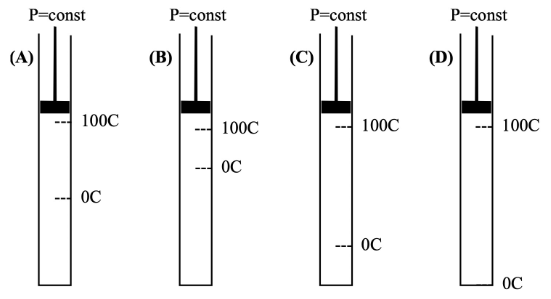
\includegraphics[width=100mm]{18.png}
	\end{figure}
	
	We are given that the pressure $P$ and the number of molecules $N$ are fixed. We will use the ideal gas law $PV=Nk_B T$ to figure out the ratio of volumes from different temperatures:
	
	$$\frac{V_{\SI{100}{\celsius}}}{V_{\SI{0}{\celsius}}}$$
	
	First we convert temperatures to its SI unit kelvins by adding $273.15$, this gives $0+273.15=\SI{273.15}{\kelvin}$ and $100+273.15=\SI{373.15}{\kelvin}$. The ratio becomes:
	
	$$\frac{V_{\SI{100}{\celsius}}}{V_{\SI{0}{\celsius}}}=\frac{\cancel{\frac{Nk_B}{P}} (\SI{373.15}{\kelvin})}{\cancel{\frac{Nk_B}{P}} (\SI{273.15}{\kelvin})}=1.3661$$
	
	It is almost $\frac43$, so the reasonable picture is (B).
\end{texample}

\begin{texample}
	Nitrogen gas ($N_2$) is compressed to $\SI{10}{\atmosphere}$ and stored in a $\SI{10}{\liter}$ cylinder at room temperature ($\SI{21}{\celsius}$). How much does the nitrogen weigh? The molar mass of a \textit{single} nitrogen atom is $\SI{14}{\gram\per\mole}$. \\
	
	We are given that
	
	$$P=\SI{10}{\atmosphere}=\SI{1e6}{\pascal}$$
	$$T=273.15+21=\SI{294.15}{\kelvin}$$
	$$V=\SI{10}{\liter}=\SI{10e-3}{\cubic\meter}$$
	$$M_{N_2}=\SI{28}{\gram\per\mole}$$
	
	We use the ideal gas law $PV=nRT$ to calculate the amount of Nitrogen $n$:
	
	$$n=\frac{PV}{RT}=\SI{4.13}{\mole}$$
	
	The mass of the gas is therefore
	
	$$m=nM_{N_2}=\SI{116}{\gram}$$
\end{texample}

\subsection{Degrees of Freedom and Equipartition Theorem}

\subsubsection{Introduction}

Ideal gases contain kinetic energy only but not all gases in the real world are ideal because they have other forms of energy. The total thermal energy of a real gas contains the following terms:

$$U_{tot}=U_k+U_{rot}+U_{vib}+U_g+U_{int}+U_{chem}+U_{rest}$$

where $U_k$ is kinetic energy, $U_{rot}$ is rotational kinetic energy, $U_g$ is gravitational potential\footnote{We don't typically include $U_g$ because the effects of gravitational potential are very small compared to kinetic energy, so they can be neglected. This approximation works for gases on ground level but for gases in the atmosphere, gravity must be taken in account.}, $U_{int}$ is interaction energy, $U_{chem}$ is chemical energy, $U_{rest}$ is rest energy. There could be more forms of energy we forgot to add. \\

In the context of thermal physics, degrees of freedom refers to the number of ways a particle can store energy. For monoatomic particles in an ideal gas, there are three translational degrees of freedom, each specified by $v_x$, $v_y$ and $v_z$. The other degrees of freedom include rotational motion, vibration, etc. For these types of energy, the formulas take the following forms:

$$\frac12mv_x^2, \quad \frac12mv_y^2, \quad \frac12mv_z^2, \quad \frac12I\omega^2, \quad \frac12kx^2, \quad \dots$$

We see that they all share the same format $\frac12cx^2$ where $c$ is some constant and $x^2$ is some (quadratic) degree of freedom. We will calculate the average energy at temperature $T$ of any degree of freedom. \\

We start by calculating the partition function for a degree of freedom:

$$Z=\frac{1}{\Delta x}\int_{-\infty}^\infty dx e^{-\beta\frac{c}{2}x^2}=\frac{1}{\Delta x}\left(\frac{2}{\beta c}\right)^\frac12 \int_{-\infty}^\infty du \: e^{-u^2}=\frac{1}{\Delta x}\left(\frac{2\pi}{\beta c}\right)^\frac12$$

Next, the average energy of a degree of freedom is:

$$\langle E \rangle=\frac12c\langle x^2 \rangle=\frac{c}{2}\frac{1}{\Delta x}\int_{-\infty}^\infty dx \: x^2 \frac{e^{-\beta\frac{c}{2}x^2}}{Z}=\left(\frac{\beta c}{2\pi}\right)^\frac12\left(\frac{2}{\beta c}\right)^\frac12 \frac{1}{\beta} \int_{-\infty}^\infty du \: u^2 e^{-u^2}=\frac{1}{2\beta}=\frac12k_BT$$

Notice the energy is independent of $c$. This important result is known as the equipartition theorem. It states that at temperature $T$, the system's thermal energy is equally divided in all degrees of freedom in such way that the average energy of each degree of freedom is

$$\frac12cx^2=\frac12k_BT$$

For a particle with $f$ degrees of freedom, its average energy is

$$\langle E \rangle=\frac{f}{2}k_BT$$

For a system with $N$ particles with $f$ degrees of freedom, its total \textit{thermal} energy is

$$U_{tot}=N\langle E \rangle=\frac{f}{2}Nk_BT$$

As a side note, this equation allows us to express temperature in terms of average energy:

$$T=\frac{2}{fk_B}\langle E \rangle$$

We see that temperature increases as particles' average energy increases (by moving faster for instance).

\subsubsection{Degrees of Freedom of Various Molecules}

Besides monoatomic molecules (\ce{He}, \ce{Ne}, etc.), there are also diatomic (\ce{N2}, \ce{O2}, etc.) and triatomic molecules (\ce{H2O}, \ce{CO2}, etc.) which have more than three degrees of freedom. The below table summarizes the number of degrees of freedom in 2D for each molecule type at room temperature.

\begin{center}
	\begin{tabular}{|l|c|l|}
		\hline
		Type & \# of Degrees of Freedom & Types of Degrees of Freedom \\
		\hline
		Monoatomic & 2 & 2 translational \\
		\hline
		Diatomic & 3 & 2 translational, 1 rotational \\
		\hline
		Triatomic & 3 & 2 translational, 1 rotational \\
		\hline
	\end{tabular}
\end{center}

Here is the table for 3D

\begin{center}
	\begin{tabular}{|l|c|l|}
		\hline
		Type & \# of Degrees of Freedom & Types of Degrees of Freedom \\
		\hline
		Monoatomic & 3 & 3 translational \\
		\hline
		Diatomic & 5 & 3 translational, 2 rotational \\
		\hline
		Triatomic & 6 & 3 translational, 3 rotational \\
		\hline
	\end{tabular}
\end{center}
\begin{figure}[h!]
	\centering
	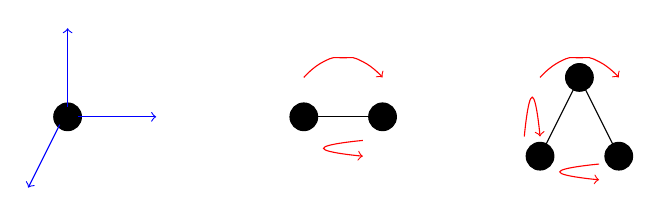
\begin{tikzpicture}
		\filldraw[fill=black, draw=black] (0,0) circle (5pt);
		\draw[->, blue] (0.13,0) -- (1.125,0);
		\draw[->, blue] (0,0.13) -- (0,1.125);
		\draw[->, blue] (-0.1,-0.1) -- (-0.5,-0.9);
		
		\filldraw[fill=black, draw=black] (3,0) circle (5pt);
		\filldraw[fill=black, draw=black] (4,0) circle (5pt);
		\draw[black] (3,0) -- (4,0);
		\draw[->, red] plot [smooth, tension=1] coordinates {(3,0.5) (3.25,0.7) (3.5,0.75) (3.75,0.7) (4,0.5)};
		\draw[->, red] plot [smooth, tension=1] coordinates {(3.75,-0.3) (3.25,-0.4) (3.75,-0.5)};
		
		\filldraw[fill=black, draw=black] (6,-0.5) circle (5pt);
		\filldraw[fill=black, draw=black] (7,-0.5) circle (5pt);
		\filldraw[fill=black, draw=black] (6.5,0.5) circle (5pt);
		\draw[black] (6,-0.5) -- (6.5,0.5);
		\draw[black] (7,-0.5) -- (6.5,0.5);
		\draw[->, red] plot [smooth, tension=1] coordinates {(6,0.5) (6.25,0.7) (6.5,0.75) (6.75,0.7) (7,0.5)};
		\draw[->, red] plot [smooth, tension=1] coordinates {(6.75,-0.6) (6.25,-0.7) (6.75,-0.8)};
		\draw[->, red] plot [smooth, tension=1] coordinates {(5.8,-0.25) (5.9,0.25) (6,-0.25)};
		
	\end{tikzpicture}
	\caption{Visualization of the degrees of freedom of monoatomic, diatomic, and triatomic molecules in 3D. Monoatomic molecules only have three translational degrees of freedom (specified by velocities $v_x,v_y,v_z$), diatomic molecules have three translational plus two rotational degrees (it cannot rotate along the rotation axis parallel to its length due to quantum mechanical reasons), and the triatomic molecules have three translational and rotational degrees of freedom each.}
\end{figure}

Intramolecular bonds in diatomic and triatomic molecules can also vibrate like springs. The reason we didn't include vibrational degrees of freedom in the table above is that vibrational modes are, in some sense, frozen out at room temperature but once the temperature is high enough, vibrational modes do need to be taken into account. Vibrational modes are excited only if the room's temperature is high enough to overcome the energy gap between the ground and first excited state for that degree of freedom (ie. $\Delta E < \frac12k_BT$). When vibration is taken into account, it will count as two degrees of freedom - one for spring kinetic energy and one for spring potential energy. There are also other modes of vibration besides stretching: twisting or flexing and they each count as two degrees of freedom. \\

The frozening of degrees of freedom can be explained using quantum mechanics. Degrees of freedom that are not in the classical regime can be described as ``frozen out'' (frozen at their quantum zero state) and don’t contribute to the total energy. At low temperatures gas molecules only have translational degrees of freedom, then as they gain more energy they can also have rotational degrees of freedom, and then at really high temperatures they can also have vibrational degrees of freedom. But at those temperatures they have so much energy the molecules just break apart into plasma, so those vibrational degrees of freedom don't really exist classically for gases.

\begin{figure}[H]
	\centering
	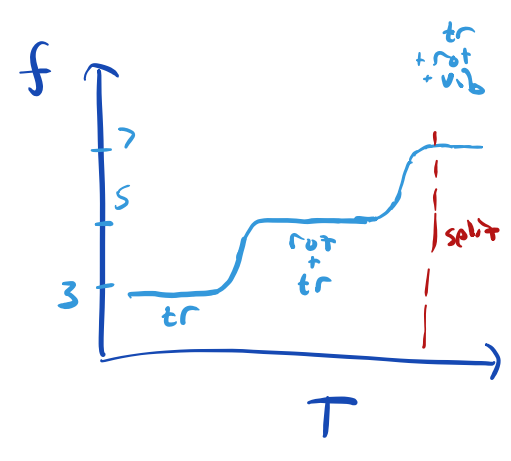
\includegraphics[width=100mm]{22.png}
	\caption{Graph showing the relationship between DoF and temperature. The red line is where molecules ionize to become plasma.}
\end{figure}

The frozening of degrees of freedom also explains why we don't typically take in account of rest-mass energies, or chemical energy stored in the molecular bonds. They are frozen at their quantum mechanical values unless the temperature is high enough for the gas to ionize.

\begin{texample}
	How many degrees of freedom does a diatomic molecule in gas exposed to high temperature have in two dimensions? Find the total energy for each diatomic molecule. \\
	
	There are $2$ translational degrees of freedom $v_x,v_y$ for center of mass to move independently in x and y directions, $1$ rotational degree of freedom to rotate on xy plane, and $2$ vibrational degrees of freedom: spring kinetic energy term and spring potential energy term. So there are $f=5$ degrees of freedom in total. The total energy for a diatomic molecule is:
	
	$$E=\underbrace{\frac12M(v_x^2+v_y^2)}_{\text{translational}}+\underbrace{\frac12I\omega^2}_{\text{rotational}}+\underbrace{\frac12\mu \dot{x}^2+\frac12kx^2}_{\text{vibrational}}$$
	
	where $M=m_1+m_2$ is total mass, $I$ is moment of inertia, $\omega$ is angular velocity, $\mu=\frac{m_1m_2}{m_1+m_2}$ is reduced mass, $x$ is distance from spring equilibrium position, and $k$ is spring constant. \\
	
	Note in three dimensions, there is an extra translational and rotational degrees of freedom, so the total will be $f=7$.
\end{texample}

\begin{texample}
	How many degrees of freedom does a \ce{H2O} molecule have in high temperatures? \\
	
	This is an example of triatomic molecule. There are $3$ translational degrees of freedom for its CoM, $3$ rotational degrees of freedom, and $6$ vibrational degrees of freedom. Stretching of each bond contributes $2$ vibrational degrees of freedom. But the molecules can bend as well which contributes $2$ extra vibrational degrees of freedom. So the total is $f=6$.
	
	\begin{figure}[H]
		\centering
		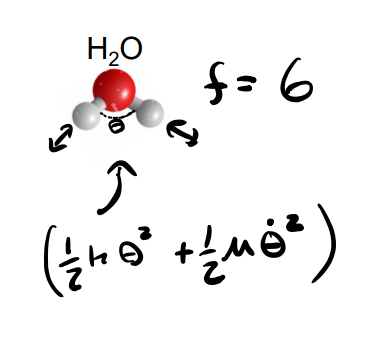
\includegraphics[width=100mm]{19.png}
		\caption{Vibrational DoFs in \ce{H2O}}
	\end{figure}
\end{texample}

\begin{texample}
	How many degrees of freedom does an atom in a solid in three dimensions have? \\
	
	An atom in a solid can't move or rotate because they are trapped in lattice with other atoms however it can vibrate in three perpendicular directions, each contributing two vibrational degrees of freedom. Unlike liquids, vibrational modes of solids are not frozen out at room temperature so they do contribute to degrees of freedom. So there is a total of $f=6$ degrees of freedom.
	
	\begin{figure}[H]
		\centering
		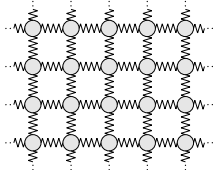
\includegraphics[width=100mm]{20.png}
		\caption{Ball-spring Model of Solid}
	\end{figure}
\end{texample}

\begin{texample}
	The vibrational energy levels of \ce{O2} are measured spectroscopically as shown. At what temperatures would \ce{O2} undertake vibrational excitations above the ground state?
	
	\begin{figure}[H]
		\centering
		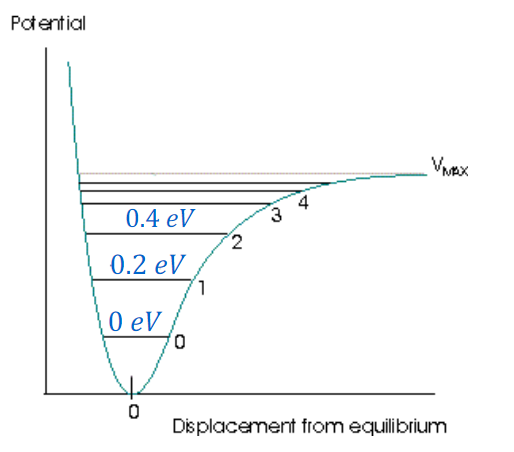
\includegraphics[width=100mm]{21.png}
	\end{figure}
	
	We can approximate using $\Delta E \approx k_BT$ where $\Delta E$ is the energy difference between the ground and first excited state. So the minimum temperature is
	
	$$T\approx\frac{\Delta E}{k_B}=\frac{\SI{0.2}{\electronvolt} (\SI{1.6e-19}{\joule\per\electronvolt})}{\SI{1.38e-23}{\joule\per\kelvin}}\approx\SI{2300}{\kelvin}$$
\end{texample}

Note on root mean square speed: this formula $v_{rms}=\sqrt{\frac{3k_BT}{m}}$ also applies to polyatomic molecules not just monoatomic gas molecules. This is because only translational DoFs contribute to gas kinetic energy.

\subsection{Work, Heat and First Law of Thermodynamics}

Work and heat are fundamentally two different things. Work is defined as a mechanical transfer of energy into or out of a system. Examples of doing work include squeezing a bottle of a gas, or pushing a piston, or shaking a hot water kettle. Heat refers to any non-mechanical transfer of energy which does no work. For example, when you boil water in a kettle, the water will heat up and gain energy but since there is no mechanical process involved, so no work is done. Remember that heat is a spontaneous flow of energy due to temperature. Other examples include how your laptop feels hot after you perform some CPU-intensive task. \\

Let $\Delta U$ be the change in energy of a system, $Q_{in}$ be the heat that flows \textit{in} the system, and $W_{on}$ the work done \textit{on} the system. The first law of thermodynamics simply states that

\[ \Delta U=Q_{in}+W_{on} \]

or the total change in energy of a system is equal to the sum of its mechanical and non-mechanical transfers of energy\footnote{Some authors prefer to define $W$ as the amount of work done \textit{by} the system and the equation would instead be \( \Delta U=Q-W \). But in this notes, we will go with $W$ defined as the work done on the system.}. Be careful with signs in this equation! $Q_{in}$ is negative if heat leaves the system and $W_{on}$ is negative if the system is being worked on. \\

It is worth noting here that while $W_{on}$ and $Q_{in}$ are both \textbf{functions of path}; how much work we do or a system does, or how much heat flows in/out of a system depends on how a process happens. However, the internal energy is a \textbf{function of state}, like the ideal gas law. The moral is that while how a system might gain or lose energy is a function of the path, the internal energy itself is a function of the state of the system only.

\begin{figure}[H]
	\centering
	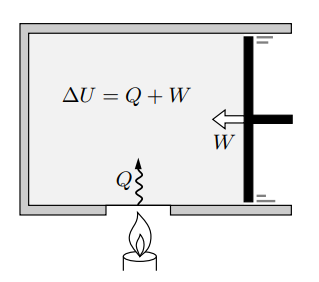
\includegraphics[width=60mm]{23.png}
	\caption{Illustration of the First Law}
\end{figure}

\subsection{Compression Work on Gas}

Work is generally defined as

$$W = \int_{x_1}^{x_2} Fdx$$

However, in thermodynamics we don't have position or force as variables to work with. Instead, we have pressure and volume. Force due to pressure is $F = PA$ and we substitute it into the equation we get

$$W = \int_{x_1}^{x_2} PAdx$$

The product of area and distance is volume. So, since $dx$ is a tiny displacement, which ultimately is a length, $Adx$ is a tiny change in volume! Note that we are assuming that volume changes are quasistatic (slow) so that pressure is equally distributed throughout the gas. Therefore:

$$W = \int_{V_1}^{V_2} PdV$$

However, this work was based on the definition of the amount of work done \textbf{by} a system on another system. We want the amount of work done \textbf{on} the system. Due to the conservation of energy, we can just throw a negative sign in front to get

$$W_{on} = -\int_{V_1}^{V_2} PdV$$

This is the proper definition of the work done on a gas. Note that since pressure $P$ can change with volume so $P$ is a function of volume. But if pressure is constant, the work becomes

$$ W_{on} = -P\int_{V_1}^{V_2}dV = -P \Delta V$$

It also applies when $\Delta V$ is infinitesimally small.

\begin{figure}[H]
	\centering
	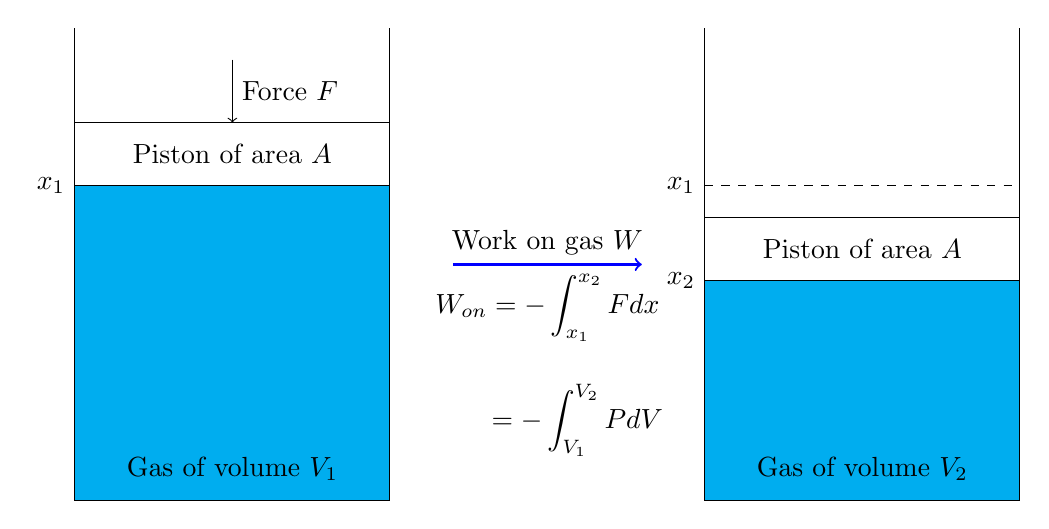
\begin{tikzpicture}[scale=4]
		\filldraw[fill=cyan, draw = black] (0,0) rectangle (1,1);
		\draw[black] (0,1) rectangle (1,1.2);
		\draw (0,1.2) -- (0,1.5);
		\draw (1,1.2) -- (1,1.5);
		\draw[->] (0.5,1.4) -- (0.5,1.2);
		\node[right] at (0.5,1.3) {Force $F$};
		\node[left] at (0,1) {$x_1$};
		\draw (0.5,0.1) node {Gas of volume $V_1$};
		\draw (0.5, 1.1) node {Piston of area $A$};
		\draw[->, blue, thick] (1.2,0.75) -- (1.8, 0.75);
		\node[above] at (1.5,0.75) {Work on gas $W$};
		\node[below] at (1.5,0.75) {$\displaystyle W_{on} = -\int_{x_1}^{x_2} Fdx$};
		\node[below] at (1.5,0.4) {$\displaystyle \phantom{W_{on}} = -\int_{V_1}^{V_2} PdV$};
		\filldraw[fill=cyan, draw = black] (2,0) rectangle (3,0.7);
		\draw[black] (2,0.7) rectangle (3,0.9);
		\draw[dashed] (2,1) -- (3,1);
		\draw (2,1.5) -- (2,0.9);
		\draw (3,1.5) -- (3,0.9);
		\node[left] at (2,1) {$x_1$};
		\node[left] at (2,0.7) {$x_2$};
		\draw (2.5,0.1) node {Gas of volume $V_2$};
		\draw (2.5, 0.8) node {Piston of area $A$};
	\end{tikzpicture}
	\caption{Illustration of Gas Being Compressed}
\end{figure}

\begin{texample}
	In the setup shown below, the gas inside is kept at constant pressure and temperature. The right piston slowly lowers and left piston slowly raises, while the pressure and temperature inside is kept constant. What is the net work done on the gas? 
	
	\begin{figure}[H]
		\centering
		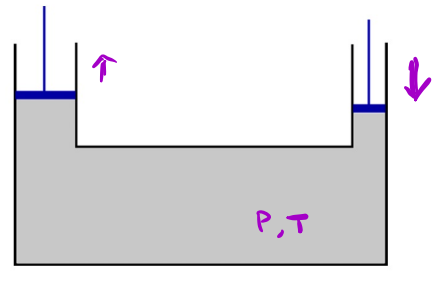
\includegraphics[width=60mm]{24.png}
	\end{figure}
	
	Since the volume does not change, the net work done on the gas is $W_{on}=-P\Delta V=0$.
\end{texample}

\begin{texample}
	Assuming the same setup from the previous example: The right piston slowly lowers and left piston slowly raises, while the pressure and temperature inside is kept constant. Ignoring friction (so that the system doesn't lose energy from heat), what do you say about external forces acting on either piston? What about work? \\
	
	External forces\footnote{If it is vacuum in the surroundings, it will point up and the pistons will explode outwards but it is not the case here} acting on either piston are pointing down all the time, both with the same magnitude: $F_L=F_R$. The total work applied to this system is still zero:
	
	$$W=F_L\Delta x_L +F_R\Delta x_R=0$$
	
	In the case when $A_L=A_R$, we have $\Delta x_L=-\Delta x_R$ and $v_L = -v_R$\footnote{Note that force balance does not necessarily imply $v=0$. Zero acceleration means constant velocity.} at some time.
\end{texample}

\subsection{PV Diagrams}

Pressure-Volume (PV) diagrams are the nice way to illustrate various thermodynamic processes. Shown below is a PV graph of a thermodynamic process that takes the gas from starting temperature $T_1$ (at pressure $P_1$ and volume $V_1$) to temperature $T_2$ (at pressure $P_2$ and volume $V_2$). Of course, there's nothing stopping us from assigning numbers to $P,T,V$, as well, if the situation calls for it. The process pictured below is an expansion of the gas, but we could also very well draw the arrow the other way and depict a compression of the gas. 

\begin{figure}[H]
	\centering
	\begin{tikzpicture}
		\draw[stealth-stealth] (0,5) node[below left]{$P$} |- (5,0) node[below left]{$V$};
		\draw[thick,->] (1,4) -- (2.5,2.5);
		\draw[thick] (2.5,2.5) -- (4,1);
		\draw[dashed] (4,0) -- (4,1);
		\draw[dashed] (1,0) -- (1,4);
		\draw[dashed] (4,1) -- (0,1);
		\draw[dashed] (1,4) -- (0,4);
		\filldraw (1,4) circle (2pt);
		\filldraw (4,1) circle (2pt);
		\node[below] at (1,0) {$V_1$};
		\node[below] at (4,0) {$V_2$};
		\node[left] at (0,1) {$P_2$};
		\node[left] at (0,4) {$P_1$};
		\node[right] at (1,4) {$T_1$};
		\node[right] at (4,1) {$T_2$};
	\end{tikzpicture}
	\caption{PV Diagram for Gas Expansion}
\end{figure}

In the previous section, we defined the work done on the gas as:

\[ W_{on} = -\int_{V_1}^{V_2} PdV \]

And looking at the PV diagram, it now becomes clear that this is nothing more than the (negative) area under the PV curve! As an example, let's figure out the work done on the gas in the process shown above. All we have to do is calculate the area underneath the curve. For convenience, let us split it into two parts of the triangle and the rectangle. For the triangle, we have area $\frac{1}{2}\left(P_1-P_2\right)\left(V_2-V_1\right)$, and for the rectangle, we have area $P_2\left(V_2-V_1\right)$. Therefore, the total area under the graph is:

\[ \text{Area } = \frac{1}{2}\left(P_1-P_2\right)\left(V_2-V_1\right) + P_2\left(V_2-V_1\right) = \frac{1}{2}\left[\left(P_1+P_2\right)\left(V_2-V_1\right) \right]\]

This area is in fact the work done \textbf{by} the gas, and the work done on the gas is just its negative:

\[W_{on} = \frac{1}{2}\left[\left(P_1+P_2\right)\left(V_1-V_2\right) \right]\]

When using this area argument, do be careful of which direction the curve is going; for example, if the process was a compression of the gas rather than an expansion, we would have to introduce a negative sign as things would be going in the opposite direction.

\begin{texample}
	A thermodynamic system, close to equilibrium, follows a closed path on the PV diagram in the direction shown. Consider one full cycle, starting and ending at the blue dot. Is the total net heat added to the system over the course of this cycle \(Q_{in}\) less than, greater than, or equal to zero?
	
	\begin{figure}[H]
		\centering
		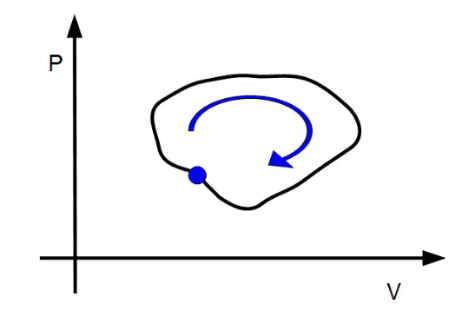
\includegraphics[width=60mm]{25.png}
	\end{figure}
	
	Since the system start and end at the same point, \(U_i=U_f\) which means the change of energy \(\Delta U=0\). According to the first law of thermodynamics,
	
	\[ Q_{in}=-W_{on} \]
	
	\begin{figure}[H]
		\centering
		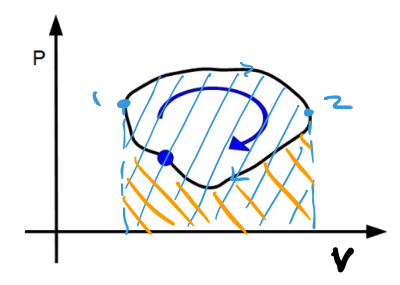
\includegraphics[width=60mm]{26.png}
	\end{figure}
	
	\(W_{on}\) is the sum of the work on the system to get from point 1 to point 2 and the work on the system to get from point 2 to point 1:
	
	\[W_{on}=W_{1\to2}+W_{2\to1}\]
	\[W_{on}=-\textcolor{cyan}{A_{1\to2}}+\textcolor{orange}{A_{2\to1}}\]
	
	$Q_{in}$ is
	
	\[ Q_{in}=-W_{on}=\textcolor{cyan}{A_{1\to2}}-\textcolor{orange}{A_{2\to1}} \]
	
	Therefore \(Q_{in}\) is greater than zero.
\end{texample}

\begin{texample}
	Imagine some helium in a cylinder with an initial volume of $\SI{1}{\liter}$ and an initial pressure of $\SI{1}{\atmosphere}$. Somehow the helium is made to expand to a final volume of $\SI{3}{\liter}$ (like by increasing temperature during process), in such a way that its pressure rises in direct proportion to its volume. Calculate the amount of heat added to the helium. \\
	
	We have
	
	\[V_1=\SI{0.001}{\cubic\meter}\]
	\[V_2=\SI{0.006}{\cubic\meter}\]
	\[P_1=\SI{101325}{\pascal}\]
	
	The PV diagram for the process is shown below:
	
	\begin{figure}[H]
		\centering
		\begin{tikzpicture}
			\draw[stealth-stealth] (0,5) node[below left]{$P$} |- (5,0) node[below left]{$V$};
			\draw[thick,->] (1,1) -- (2.5,2.5);
			\draw[thick] (2.5,2.5) -- (4,4);
			\draw[dashed] (4,0) -- (4,4);
			\draw[dashed] (1,0) -- (1,1);
			\draw[dashed] (0,1) -- (1,1);
			\draw[dashed] (0,4) -- (4,4);
			\filldraw (1,1) circle (2pt);
			\filldraw (4,4) circle (2pt);
			\node[below] at (1,0) {$V_1$};
			\node[below] at (4,0) {$V_2$};
			\node[left] at (0,1) {$P_1$};
			\node[left] at (0,4) {$P_2$};
		\end{tikzpicture}
	\end{figure}
	
	We are given that $P(V)=cV$ where $c$ is some constant. The constant is calculated with the given initial condition:
	
	\[c=\frac{P_1}{V_1}=\SI{10132500}{\pascal\per\cubic\meter}\]
	
	$P_2$ is calculated as follows:
	
	\[P_2=cV_2=\SI{607950}{\pascal}\]
	
	With all pieces in place, we calculate the work done on the gas:
	
	\[W_{on}=-\int_{V_1}^{V_2} cVdV=-c\left( \frac{V_2^2}{2} - \frac{V_1^2}{2} \right)=\SI{-1773.1875}{\joule}\]
	
	The change in helium's internal energy is:
	
	\[\Delta U=\frac{3}{2}\Delta(PV)=\frac{3}{2}(P_2V_2-P_1V_1)=\SI{5319.5625}{\joule}\]
	
	The heat added to the gas by the first law of thermodynamics is therefore:
	
	\[Q=\Delta U-W_{on}=\SI{7092.75}{\joule}\]
	
\end{texample}

\subsection{Thermodynamic Processes}

\subsubsection{Isochoric Process}

Isochoric processes are heating/cooling processes where the volume of the gas does not change ($\Delta V = 0$). For example, when you heat the gas sealed in a jar, the gas does not change its volume since the jar walls are rigid but its energy changes. $V$ does not change but $P$ and $T$ changes. \\

On a PV diagram, isochoric processes look like a straight vertical line. As the gas gets heated up, the volume of the gas remains unchanged, so the process should be a graph of a line with constant $V$. Conversely, as the gas goes from a lower temperature $T_1$ to a higher temperature $T_2$, we would expect the pressure to increase.

\begin{figure}[H]
	\centering
	\begin{tikzpicture}
		\draw[stealth-stealth] (0,5) node[below left]{$P$} |- (5,0) node[below left]{$V$};
		\draw[thick,->] (2.5,1) -- (2.5,2.5);
		\draw[thick] (2.5,2.5) -- (2.5,4);
		\draw[dashed] (2.5,1) -- (2.5,0);
		\draw[dashed] (2.5,1) -- (0,1);
		\draw[dashed] (2.5,4) -- (0,4);
		\filldraw (2.5,1) circle (2pt);
		\filldraw (2.5,4) circle (2pt);
		\node[below] at (2.5,0) {$V_1$};
		\node[left] at (0,1) {$P_1$};
		\node[left] at (0,4) {$P_2$};
		\node[right] at (2.5,1) {$T_1$};
		\node[right] at (2.5,4) {$T_2$};
	\end{tikzpicture}
	\caption{PV Diagram for Isochoric Process}
\end{figure}

Since a straight vertical line has no area, the work done on the gas during the process is

$$W=-\int_{V_1}^{V_2}PdV=0$$

since there is no change in volume. According to the first law of thermodynamics,

$$\Delta U=Q+W=Q$$

The change in internal energy is just the heat that flows in/out of the system. We can express it in terms of temperature change:

$$\Delta U=\frac{f}{2}Nk_B\Delta T=Q$$

We define the quantity $C$ heat capacity:

$$C=\frac{Q}{\Delta T}$$

This is the heat needed to change the temperature of a system by one degree, or the ratio of the heat added to the system to the change in temperature. \\

For isochoric processes, we have heat capacity at the \textbf{fixed volume} for ideal gases:

$$C_v=\frac{f}{2}Nk_B$$

We obtain heat as a function of the change in temperature and amount (and degrees of freedom!) of the gas:

$$Q=C_v \Delta T$$

\subsubsection{Isobaric Process}

Isobaric processes are compression/expansion processes in which the pressure of the gas does not change ($\Delta P = 0$). For example, consider a box of gas where the top face is covered by a massless piston that slides without friction. If the gas heats up slowly then the piston gets pushed up slowly\footnote{The piston should rise slowly (or quasistatically) so that the gas pressure matches the surroundings.} by the warming, expanding gas, while the pressure of the gas stays constant. $P$ stays constant but $V$ and $T$ increases. Heating a balloon is another example of an isobaric process. It heats up while it warms up and expands. The pressure inside the balloon matches the surroundings.

\begin{figure}[H]
	\centering
	\begin{tikzpicture}
		\draw[stealth-stealth] (0,5) node[below left]{$P$} |- (5,0) node[below left]{$V$};
		\draw[thick,->] (1,2.5) -- (2.5,2.5);
		\draw[thick] (2.5,2.5) -- (4,2.5);
		\draw[dashed] (0,2.5) -- (1,2.5);
		\draw[dashed] (1,0) -- (1,2.5);
		\draw[dashed] (4,0) -- (4,2.5);
		\filldraw (1,2.5) circle (2pt);
		\filldraw (4,2.5) circle (2pt);
		\node[below] at (4,0) {$V_2$};
		\node[below] at (1,0) {$V_1$};
		\node[left] at (0,2.5) {$P_1$};
		\node[above] at (1,2.5) {$T_1$};
		\node[above] at (4,2.5) {$T_2$};
	\end{tikzpicture}
	\caption{PV Diagram for Isobaric Process}
\end{figure}

The work done in this process is just

$$W=-P\Delta V$$

since the pressure is constant. Applying the ideal gas law, the change in temperature is

$$\Delta T = \frac{P}{Nk_B}\Delta V$$

and the change in internal energy is

$$\Delta U = \frac{f}{2}Nk_B\Delta T=\frac{f}{2}P\Delta V$$

The amount of heat added to the gas is calculated using the first law of thermodynamics:

$$Q=\Delta U-W=\frac{f+2}{2} P\Delta V$$

is related to temperature by

$$Q=\frac{f+2}{2} Nk_B\Delta T$$
$$Q=C_p\Delta T$$

We also found the formula for heat capacity at the \textbf{fixed pressure}:

$$C_p=\frac{f+2}{2} Nk_B$$

Note that $C_p > C_v$, or that the heat capacity at constant pressure is higher than the heat capacity at constant volume for gases. This tells us that when gas is allowed to expand as it is heated (retaining constant pressure), it requires more energy to increase its temperature than if it is kept at a fixed volume.

\begin{texample}
	Consider $\SI{1}{\cubic\centi\meter}$ of methane (\ce{CH4}) gas at $\SI{2}{\atmosphere}$ of pressure and at temperature equal to $\SI{25}{\celsius}$. A molecule of methane has tetrahedral shape. Find the amount of heat that has to be removed while compressing the gas to $\SI{0.4}{\cubic\centi\meter}$ to stop the pressure from rising. \\
	
	This is an isobaric process. We have
	
	$$\Delta V=\SI{-0.6}{\cubic\centi\meter}=\SI{-6e-7}{\cubic\meter}$$
	
	$$P=\SI{2}{\atmosphere}=\SI{202650}{\pascal}$$
	
	$$f=6$$
	
	Applying the first law of thermodynamics,
	
	$$Q=\Delta U - W=\frac{f}{2}Nk_B\Delta T - W=\frac{f}{2}P\Delta V+P\Delta V=\frac{f+2}{2}P\Delta V=\SI{-0.49}{\joule}$$
\end{texample}

\subsubsection{Isothermal Process}

Isothermal processes are compression/expansion processes in which the temperature of the gas remains constant ($\Delta T = 0$). These processes occur very slowly. As an example, consider a box of gas where the top face is a piston again. When the piston is pushed down very very slowly, the gas inside the piston remains at thermal equilibrium with its surroundings. Hence, as we do work on the gas, an equal amount of energy leaves the gas in the form of heat, and the gas inside the piston stays at the same temperature.

\begin{figure}[H]
	\centering
	\begin{tikzpicture}
		\begin{axis}[
			axis x line=bottom,
			axis y line=left,
			xmin=0, xmax=10,
			ymin=0, ymax=10,
			%        % (made labels more common)
			%        % (because of the "sketch" type of the plot these should not be needed)
			%        xlabel={Volume $(\mathrm{m}^3)$},
			%        ylabel={Pressure (Pa)},
			% (changed ticks + labels to normal ticks instead of extra ticks)
			xtick={3,6},
			xticklabels={$V_2$,$V_1$},
			ytick={1.5,6},
			yticklabels={$P_1$,$P_2$},  % <-- (changed order of entries)
			]
			% fill the area below the curve
			% (draw it first, so it is below everything else)
			
			
			% draw the dashed lines
			% (using two different approaches)
			\addplot [dashed,domain=0:3,samples=2] {6};
			\addplot [dashed,domain=0:6,samples=2] {1.5};
			
			\draw [dashed,thin] (axis cs:6,1.5) -- (axis cs:6,0);
			\draw [dashed,thin] (axis cs:3,6)   -- (axis cs:3,0);
			
			% now draw the curve
			\draw [
			fleche={0.6:black},              % <-- added
			] (axis cs:6,1.5) to [bend left=30]
			% store start and end coordinates
			coordinate [pos=0] (start)
			coordinate [pos=1] (end)
			(axis cs:3,6);
			
			% draw start and end point
			\fill [radius=2pt]
			(start) circle[]
			(end)   circle[];
		\end{axis}
		\node[below] at (6.5,0) {$V$};
		\node[left] at (0,5.5) {$P$};
		\node[right] at (2.2,3.4) {$T_2$};
		\node[right] at (4.25,0.9) {$T_1$};
	\end{tikzpicture}
	\caption{PV Diagram for Isothermal Compression}
\end{figure}

The relationship between pressure and volume according to the ideal gas law is

$$P=\frac{Nk_BT}{V}$$

The work done on the gas during this process is

$$W=-\int_{V_1}^{V_2} \frac{Nk_BT}{V} dV = -Nk_BT \int_{V_1}^{V_2}\frac{1}{V}dV = Nk_BT\ln\left( \frac{V_1}{V_2} \right)$$

Since there is no temperature change, the change in internal energy is zero\footnote{For ideal gases, this is true but for real gases, this is not always true. Change in internal energy $U$ contains many other factors like pressure.}:

$$\Delta U = \frac{f}{2}Nk_B\Delta T = \frac{f}{2} (P \Delta V + V\Delta P) = 0$$

\footnote{$\Delta(PV)=P \Delta V + V\Delta P$ arises from product rule. $P \Delta V + V\Delta P$ is equal to zero because $\frac{dV}{dP}=\frac{d}{dP}\left( \frac{Nk_BT}{P} \right)=-\frac{Nk_BT}{P^2}$ and $P\Delta V=P\left(-\frac{Nk_BT}{P^2}\Delta P\right)=-\frac{Nk_BT}{P}\Delta P=-V\Delta P$ which cancels out the $V\Delta P$ term} From the first law of thermodynamics, it follows that

$$Q=-W=Nk_BT\ln\left( \frac{V_2}{V_1} \right)$$

\begin{texample}
	$\SI{4}{\mole}$ if ideal gas is compressed at $\SI{0}{\celsius}$ so that the volume decreases by a factor of $3$. How much work is done on the gas? \\
	
	This is an isothermal process. The work done is
	
	$$W=Nk_BT\ln\left( \frac{V_i}{V_f} \right)=Nk_BT\ln\left( 3 \right)=nRT\ln(3)=\SI{9980}{\joule}$$
\end{texample}

\subsubsection{Adiabatic Process}

Adiabatic processes are compression/expansion processes in which the gas has no heat flow ($Q=0$). These processes tend to be either fast, or occur under insulated conditions; for example, consider the same gas cylinder with the piston we discussed in the isothermal section. If instead of pushing in the piston very slowly, we push down forcefully, the compression will occur so quickly that there wouldn't be time for heat to flow out of the gas. This would be an adiabatic compression. As another example, if we had a cylinder of gas surrounded with thermal insulation, then even if we were to compress the piston or let the gas expand, there would be no heat flow and again we would have an adiabatic process. \\

Considering infinitesimal change in volume $\Delta V$, the work done in this process is

\[W=-\int_{V_0}^{V_0+\Delta V} PdV=-P\Delta V=-\frac{Nk_BT}{V} \Delta V\]

The change in internal energy is just $\Delta U=W$ since $Q=0$ which gives

\[\Delta U=\frac{f}{2}Nk_B\Delta T=-\frac{Nk_BT}{V} \Delta V\]
\[\frac{f}{2}\Delta T=-\frac{T}{V}\Delta V\]

For infinitesimal $\Delta V$ and $\Delta T$, we get the following differential equation:

\[\frac{f}{2}\frac{dT}{T}=-\frac{dV}{V}\]

Integrating both sides from initial to final state gives

\[\frac{f}{2}\int_{T_1}^{T_2}\frac{dT}{T}=-\int_{V_1}^{V_2}\frac{dV}{V}\]
\[\frac{f}{2}\ln\left(\frac{T_2}{T_1}\right)=-\ln\left(\frac{V_2}{V_1}\right)\]

\[\ln\left( \left(\frac{T_2}{T_1}\right)^{\frac{f}{2}} \right)=\ln\left(\frac{V_1}{V_2}\right)\]

\[ \left(\frac{T_2}{T_1}\right)^{\frac{f}{2}}=\frac{V_1}{V_2} \]

We conclude that

\[V_1T_1^\frac{f}{2}=V_2T_2^\frac{f}{2}\]

or

\[VT^\frac{f}{2}=\text{const}\]

\begin{figure}[H]
	\centering
	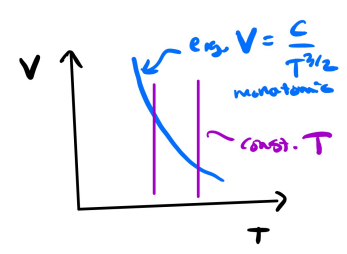
\includegraphics[width=60mm]{30.png}
	\caption{VT graph for adiabatic transform}
\end{figure}

There is the alternative form for this equation. We apply the ideal gas law $PV=Nk_BT$ to eliminate temperatures $T_1$ and $T_2$ which gives

\[V_1\left(\frac{P_1V_1}{Nk_B}\right)^\frac{f}{2}=V_2\left(\frac{P_2V_2}{Nk_B}\right)^\frac{f}{2}\]

\[P_1^\frac{f}{2} V_1^{1+\frac{f}{2}}=P_2^\frac{f}{2} V_2^{1+\frac{f}{2}}\]

Raising both sides to the power of $\frac{2}{f}$ gives

\[P_1 V_1^{\frac{2}{f}+1}=P_2 V_2^{\frac{2}{f}+1}\]

Denote constant $\gamma=\frac{2}{f}+1=\frac{f+2}{f}$ to be adiabatic index\footnote{It turns out that in general $\gamma=\frac{C_p}{C_v}$. The adiabatic index is just the ratio of heat capacity in constant pressure and heat capacity in constant volume. We see that it is true for ideal gases: $\gamma=\frac{\frac{f+2}{2}Nk_B}{\frac{f}{2}Nk_B}=\frac{f+2}{f}$}, we conclude that

\[PV^\gamma=\text{const}\]

\[V^{\gamma-1}T=\text{const}\]

So, an adiabatic curve on a PV diagram obeys the following equation

\[P=\frac{\text{const}}{V^\gamma}\]

Since $\gamma>1$, an adiabatic curve looks quite a bit like the isothermal curve, but is steeper/lies above it.

\begin{figure}[H]
	\centering
	\begin{tikzpicture}
		\begin{axis}[
			axis x line=bottom,
			axis y line=left,
			xmin=0, xmax=10,
			ymin=0, ymax=10,
			% % (made labels more common)
			% % (because of the "sketch" type of the plot these should not be needed)
			% xlabel={Volume $(\mathrm{m}^3)$},
			% ylabel={Pressure (Pa)},
			% (changed ticks + labels to normal ticks instead of extra ticks)
			xtick={3.75,6},
			xticklabels={$V_2$,$V_1$},
			ytick={1.5,6},
			yticklabels={$P_1$,$P_2$}, % <-- (changed order of entries)
			]
			% fill the area below the curve
			% (draw it first, so it is below everything else)
			
			
			% draw the dashed lines
			% (using two different approaches)
			\addplot [dashed,domain=0:3.75,samples=2] {6};
			\addplot [dashed,domain=0:6,samples=2] {1.5};
			
			\draw [dashed,thin] (axis cs:6,1.5) -- (axis cs:6,0);
			\draw [dashed,thin] (axis cs:3.75,6) -- (axis cs:3.75,0);
			
			% now draw the curve
			\draw [
			dotted,red % <-- added
			] (axis cs:3,6) to [bend right=30]
			% store start and end coordinates
			coordinate [pos=1] (start)
			coordinate [pos=0] (end)
			(axis cs:6,1.5);
			
			\draw [
			fleche={0.6:black} % <-- added
			] (axis cs:6,1.5) to [bend left=30]
			% store start and end coordinates
			coordinate [pos=0] (start)
			coordinate [pos=1] (end)
			(axis cs:3.75,6);
			
			
			% draw start and end point
			\fill [radius=2pt]
			(start) circle[]
			(end) circle[];
			\node[right] at (axis cs:6,1.5) {$T_1$};
			\node[right] at (axis cs:3.75,6) {$T_2$};
		\end{axis}
		\node[below] at (6.5,0) {$V$};
		\node[left] at (0,5.5) {$P$};
		
	\end{tikzpicture}
	\caption{PV diagram for adiabatic compression. The adiabatic curve is pictured in black, and the isothermal curve is dashed and red.}
\end{figure}

\begin{texample}
	In a Diesel engine, atmospheric air (which is mostly nitrogen gas) at temperature $\SI{22}{\celsius}$ is quickly compressed to about $1/25$ of its intial volume. Estimate the temperature of the air after compression and explain (to yourself) why a Diesel engine does not require spark plugs. \\
	
	We are given that
	
	\[T_1=\SI{295.15}{\kelvin}\]
	\[\frac{V_2}{V_1}=\frac{1}{25}\]
	\[f=5\]
	
	In any adiabatic process, $V^{\gamma-1}T=\text{const}$, so
	
	\[V_1^{\gamma-1}T_1=V_2^{\gamma-1}T_2\]
	\[\frac{T_1}{T_2}=\left( \frac{V_2}{V_1} \right)^{\gamma-1}\]
	\[T_2=\frac{T_1}{\left( \frac{V_2}{V_1} \right)^{\gamma-1}}=\frac{\SI{295.15}{\kelvin}}{\left( \frac{1}{25} \right)^{\frac{2}{5}}}=\SI{796.44}{\celsius}\]
	
	This temperature is very high!
\end{texample}

\begin{texample}
	Compute work done on a gas that starts with volume $V_1$ and pressure $P_1$, and then has its volume adiabaticaly halved. \\
	
	We have
	
	\[PV^\gamma=P_1V_1^\gamma\]
	
	The work done in this process is
	
	\begin{align*}
		W&=-\int_{V_1}^\frac{V_1}{2} PdV \\
		&=-\int_{V_1}^\frac{V_1}{2} \frac{P_1V_1^\gamma}{V^\gamma} dV \\
		&=-P_1V_1^\gamma \left[ \frac{V^{1-\gamma}}{1-\gamma} \right]_{V_1}^{\frac{V_1}{2}} \\
		&=\frac{P_1V_1^\gamma}{1-\gamma} \left[ V^{1-\gamma} \right]_{\frac{V_1}{2}}^{V_1} \\
		&=\frac{P_1V_1^{1+\frac{2}{f}}}{-\frac{2}{f}} \left[ \frac{1}{V^{\frac{2}{f}}} \right]_{\frac{V_1}{2}}^{V_1} \\
		&=-\frac{f}{2} P_1V_1^{1+\frac{2}{f}} \left[ \frac{1}{V_1^\frac{2}{f}} - \frac{2^\frac{2}{f}}{V_1^\frac{2}{f}} \right] \\
		&=\frac{f}{2} \frac{P_1V_1^{1+\frac{2}{f}}}{V_1^\frac{2}{f}} \left( 2^\frac{2}{f} - 1 \right) \\
		&=\frac{f}{2} P_1V_1 \left( 2^\frac{2}{f} - 1 \right) \\
		&=\frac{f}{2} Nk_BT_1 \left( 2^\frac{2}{f} - 1 \right)
	\end{align*}
\end{texample}

In general, work done on gas in adiabatic process is

\[W=-\int_{V_1}^{V_2} \frac{P_1V_1^\gamma}{V^\gamma} dV=P_1V_1^\gamma \frac{V_1^{1-\gamma}-V_2^{1-\gamma}}{1-\gamma}=\frac{P_1V_1-P_2V_2}{1-\gamma}=\frac{\Delta (PV)_{2\to1}}{1-\gamma}\]

The last term follows because $P_1V_1^\gamma = P_2V_2^\gamma$.

\subsection{Heat Engines}

\subsubsection{Introduction}

A heat engines is a device that receives heat energy as input and converts it into some form of useful work. We will study engines that deals with gas in this section. The outline of the process goes as follows:

\begin{enumerate}
	\item The heat engine starts in its original state.
	\item The heat engine accepts some heat $Q_H$ from an external hot bath of temperature $T_H$.
	\item The heat engine does work $W$ from the energy given to it in the form of heat.
	\item The heat engine throws away some "waste heat" $Q_C$ into a cold bath of temperature $T_C$.
	\item The heat engine returns to its original state, and the cycle begins again.
\end{enumerate}

This is demonstrated in a diagram below. Note that this is just a general outline, but really steps 2-4 can occur in a different order, multiple times, and sometimes concurrently. A diagram illustrates this below:

\begin{figure}[H]
	\centering
	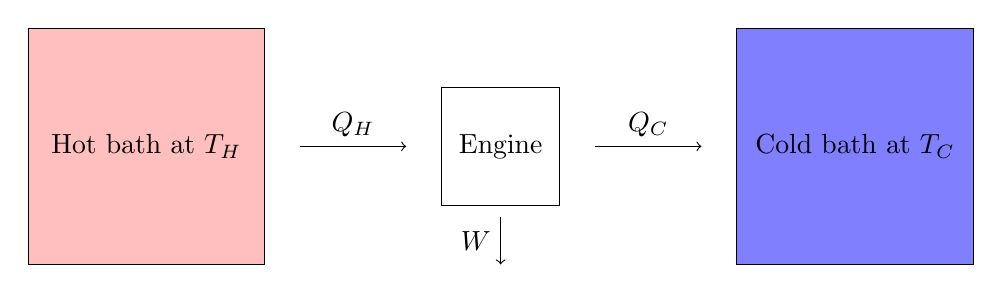
\begin{tikzpicture}[scale=3]
		\filldraw[fill=pink] (0,0) rectangle (1,1);
		\draw (1.75,0.25) rectangle (2.25,0.75);
		\filldraw[fill=blue!50] (3,0) rectangle (4,1);
		\draw[->] (1.15,0.5) -- (1.6,0.5);
		\draw[->] (2.4,0.5) -- (2.85,0.5);
		\draw[->] (2,0.2) -- (2,0);
		\node[above] at (1.375,0.5) {$Q_H$};
		\node[above] at (2.625,0.5) {$Q_C$};
		\node[left] at (2,0.1) {$W$};
		\draw (2,0.5) node {Engine};
		\draw (0.5,0.5) node {Hot bath at $T_H$};
		\draw (3.5,0.5) node {Cold bath at $T_C$};=
	\end{tikzpicture}
	\caption{Heat Engine Cartoon}
\end{figure}

Of course, we could also flip the direction in which we do things to give the opposite result, which results in a heat pump (or refrigerators). Instead of putting heat at a high temperature $T_H$ to get work $W$ out, we can instead supply the heat engine with heat $Q_C$ at a low temperature $T_C$ (which is very cheap) and then supply work to the heat engine to get heat $Q_H$ out at a high temperature. \\

To measure how good a heat engine is, we define efficiency:

\[e=\frac{W}{Q_H}\]

It can range from $0$ (where $W=0$ and we have a broken heat engine) to $1$ (where $W=Q_H$ and we have a perfect conversion of the energy we put in to the work we get out). However, we will soon see that a 100\% efficient heat engine is not realistic at all; this would require that no waste heat $Q_C$ is produced at all, which is realistically impossible. \\

The first law of thermodynamics, which is the statement of conservation of energy, for heat engines can be stated as follows:

\[Q_H=W+Q_C\]

No energy gets lost or created spontaneously during the whole process. We can rewrite the heat engine efficiency as:

\[e=\frac{Q_H-Q_C}{Q_H}=1-\frac{Q_C}{Q_H}\]

If a heat engine is very efficient ($e=1$), then there is no heat wasted (ie. $Q_C=0$). But in the real world, $e$ is always less than $1$. \\

We will study a simple heat engine, shown in the below PV diagram. The gaseous medium used in this engine is $\SI{1}{\mole}$ of ideal gas with $f$ quadratic degrees of freedom.

\begin{figure}[H]
	\centering
	\begin{tikzpicture}
		\draw[stealth-stealth] (0,5) node[below left]{$P$} |- (5,0) node[below left]{$V$};
		\filldraw (1,1) circle (2pt);
		\filldraw (4,1) circle (2pt);
		\filldraw (4,3) circle (2pt);
		\filldraw (1,3) circle (2pt);
		
		\draw[thick,->] (1,3) -- (2.5,3);
		\draw[thick] (2.5,3) -- (4,3);
		\draw[thick,->] (4,3) -- (4,2);
		\draw[thick] (4,2) -- (4,1);
		\draw[thick,->] (4,1) -- (2.5,1);
		\draw[thick] (2.5,1) -- (1,1);
		\draw[thick,->] (1,1) -- (1,2);
		\draw[thick] (1,2) -- (1,3);
		
		\node[above] at (1,3) {$3$};
		\node[above] at (4,3) {$4$};
		\node[below] at (4,1) {$1$};
		\node[below] at (1,1) {$2$};
		
		\node[below] at (4,0) {$4v$};
		\node[below] at (1,0) {$v$};
		\node[left] at (0,1) {$p$};
		\node[left] at (0,3) {$2p$};
	\end{tikzpicture}
	\caption{Simple Heat Engine}
\end{figure}

In this engine, the gas in the engine starts at state $1$, at pressure $p$ and volume $4v$. We isobarically compress the gas (by doing work on it), the gas gives off more heat in the process, until the gas reaches state $2$ at volume $v$. Then, we heat the gas isochorically, giving it heat, until it reaches state $3$ at pressure $2p$. Then, we add more heat and let it isobarically expand until it reaches state $4$ at volume $4v$. Then, we let the gas isochorically cool and give off heat until it returns to its initial state at pressure $p$. \\

We start by calculating temperatures at each state. Since we know there is $\SI{1}{\mole}$ of ideal gas, we can apply the ideal gas law: $PV=RT$ to find temperatures. We have:

\[T_1=\frac{4pv}{R}\]
\[T_2=\frac{pv}{R}\]
\[T_3=\frac{2pv}{R}\]
\[T_4=\frac{8pv}{R}\]

We see that the temperature is minimized at state $2$ but is maximized at state $4$. The ratio of maximum and minimum temperatures is:

\[\frac{T_4}{T_2}=8\]

Next, we calculate the amount of work produced by the engine to us. Note that here we want to calculate work done \textbf{by} the system (engine) \textbf{to} us, unlike the previous sections where we calculate the work done \textbf{on} the system. For example, when the engine moves from states $2$ to $4$, it does positive work to us, represented by the red area below.

\begin{center}
	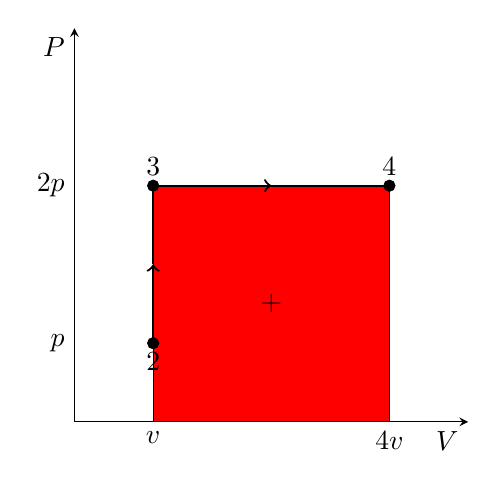
\begin{tikzpicture}
		\draw[stealth-stealth] (0,5) node[below left]{$P$} |- (5,0) node[below left]{$V$};
		\filldraw[fill=red] (1,0) rectangle (4,3);
		\draw (2.5,1.5) node {$+$};
		
		\filldraw (1,1) circle (2pt);
		%\filldraw (4,1) circle (2pt);
		\filldraw (4,3) circle (2pt);
		\filldraw (1,3) circle (2pt);
		
		\draw[thick,->] (1,3) -- (2.5,3);
		\draw[thick] (2.5,3) -- (4,3);
		%\draw[thick,->] (4,3) -- (4,2);
		%\draw[thick] (4,2) -- (4,1);
		%\draw[thick,->] (4,1) -- (2.5,1);
		%\draw[thick] (2.5,1) -- (1,1);
		\draw[thick,->] (1,1) -- (1,2);
		\draw[thick] (1,2) -- (1,3);
		
		\node[above] at (1,3) {$3$};
		\node[above] at (4,3) {$4$};
		%\node[below] at (4,1) {$1$};
		\node[below] at (1,1) {$2$};
		
		\node[below] at (4,0) {$4v$};
		\node[below] at (1,0) {$v$};
		\node[left] at (0,1) {$p$};
		\node[left] at (0,3) {$2p$};
	\end{tikzpicture}
\end{center}

The net work done by the engine is the area of the rectangular region enclosed by the cycle, as illustrated below:

\begin{center}
	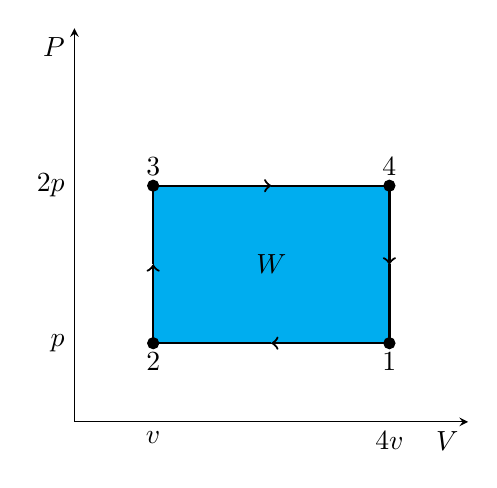
\begin{tikzpicture}
		\draw[stealth-stealth] (0,5) node[below left]{$P$} |- (5,0) node[below left]{$V$};
		\filldraw[fill=cyan] (1,1) rectangle (4,3);
		\draw (2.5,2) node {$W$};
		
		\filldraw (1,1) circle (2pt);
		\filldraw (4,1) circle (2pt);
		\filldraw (4,3) circle (2pt);
		\filldraw (1,3) circle (2pt);
		
		\draw[thick,->] (1,3) -- (2.5,3);
		\draw[thick] (2.5,3) -- (4,3);
		\draw[thick,->] (4,3) -- (4,2);
		\draw[thick] (4,2) -- (4,1);
		\draw[thick,->] (4,1) -- (2.5,1);
		\draw[thick] (2.5,1) -- (1,1);
		\draw[thick,->] (1,1) -- (1,2);
		\draw[thick] (1,2) -- (1,3);
		
		\node[above] at (1,3) {$3$};
		\node[above] at (4,3) {$4$};
		\node[below] at (4,1) {$1$};
		\node[below] at (1,1) {$2$};
		
		\node[below] at (4,0) {$4v$};
		\node[below] at (1,0) {$v$};
		\node[left] at (0,1) {$p$};
		\node[left] at (0,3) {$2p$};
	\end{tikzpicture}
\end{center}

So the net work done is therefore

\[W=(4v-v)(2p-p)=3pv\]

Applying the first law of thermodynamics:

\[\Delta U=Q-W\]

\footnote{$-W$ since we redefined work to be the one done \textbf{by} the engine.} Since $\Delta U=0$ (we will show why later in this section),

\[Q=W\]

This means all of the heat flowing into the system is converted into work done by the engine; The total heat that flows in is $Q=3pv$. Now, we will explicitly calculate heat produced/released at each state transition. Recall that heat produced at fixed volume is

\[Q=\frac{f}{2} Nk_B\Delta T\]

and for fixed pressure is

\[Q=\frac{f+2}{2} Nk_B\Delta T\]

Applying these formulas gives

\[Q_{1\to2}=\frac{f+2}{2} Nk_B(T_2-T_1)=\frac{f+2}{2} Nk_B\left(\frac{pv}{R}-\frac{4pv}{R}\right)=-\frac{f+2}{2} 3pv\]

\[Q_{2\to3}=\frac{f}{2} Nk_B(T_3-T_2)=\frac{f}{2} Nk_B\left(\frac{2pv}{R}-\frac{pv}{R}\right)=\frac{f}{2} pv\]

\[Q_{3\to4}=\frac{f+2}{2} Nk_B(T_4-T_3)=\frac{f+2}{2} Nk_B\left(\frac{8pv}{R}-\frac{2pv}{R}\right)=\frac{f+2}{2} 6pv\]

\[Q_{4\to1}=\frac{f}{2} Nk_B(T_1-T_4)=\frac{f}{2} Nk_B\left(\frac{4pv}{R}-\frac{8pv}{R}\right)=-\frac{f}{2} 4pv\]

Note that $\frac{Nk_B}{R}=\frac{N}{N_A}=n=1$. One can show that

\[Q=Q_{1\to2}+Q_{2\to3}+Q_{3\to4}+Q_{4\to1}=W\]

The overall effciency of the engine is the net work divided by the amount of heat absorbed:

\[e=\frac{W}{Q_H}=\frac{W}{Q_{2\to3}+Q_{3\to4}}=\frac{3pv}{\frac{f}{2} pv+\frac{f+2}{2} 6pv}=\frac{6}{7f+12}\]

The below table summarizes the energy flow in each state transistion.

\begin{center}
	\begin{tabular}{c|c|c|c}
		Segment & Heat & Work \textbf{by} Engine & Temperature \\
		\hline
		$1\to2$ & release & negative & decrease \\
		\hline
		$2\to3$ & absorb & none & increase \\
		\hline
		$3\to4$ & absorb & positive & increase \\
		\hline
		$4\to1$ & release & none & decrease
	\end{tabular}
\end{center}

Lastly, we show that the net change of internal energy of the whole cycle is zero. Recall that

\[U=\frac{f}{2}Nk_BT=\frac{f}{2}PV\]

The net change of the internal energy is

\begin{align*}
	\Delta U_{net} &= \Delta U_{1\to2}+\Delta U_{2\to3}+\Delta U_{3\to4}+\Delta U_{4\to1} \\
	&= \frac{f}{2}p(v-4v)+\frac{f}{2}(2p-p)v+\frac{f}{2}2p(4v-v)+\frac{f}{2}(p-2p)4v \\
	&=\frac{f}{2}(pv-4pv+2pv-pv+8pv-2pv+4pv-8pv) \\
	&=0
\end{align*}

as expected.

\subsubsection{Carnot Cycle}

The Carnot engine is more than just an engine. It is a limit on the efficiency of real-world thermodynamic processes, and was used to develop the first notions of entropy.

\begin{figure}[H]
	\centering
	\begin{tikzpicture}[
		dot/.style = {draw,fill,circle,inner sep=1pt},
		arrow inside/.style = {postaction=decorate,decoration={markings,mark=at position .55 with \arrow{>}}}
		]
		%\draw[<->] (0,6) node[above right] {$P$} |- (6,0) node[right] {$V$};
		%\draw[->] (0,0) node[above] {$P$} %|- (6,0) node[right] {$V$};
		\draw[stealth-stealth] (0,6) node[below left]{$P$} |- (6,0) node[below left]{$V$};
		\node[dot,label={right:$2$}] (@b) at (4.5,4) {};
		\node[dot,label={left:$1$}] (@a) at (1,4.5) {};
		\node[dot,label={below left:$4$}] (@d) at (1.5,1.5) {};
		\node[dot,label={right:$3$}] (@c) at (5,1) {};
		\draw[fleche={0.5:black} ] (@a) to[looseness=.7,bend right=20] (@b);
		\draw[fleche={0.5:black} ] (@b) to[looseness=.7,bend right=20] (@c);
		\draw[fleche={0.5:black} ] (@c) to[looseness=.7,bend left=20] (@d);
		\draw[fleche={0.5:black} ] (@d) to[looseness=.7,bend left=20] (@a);
	\end{tikzpicture}
	\caption{Carnot Cycle}
\end{figure}

If we start at state $1$ in the diagram, the engine first undergoes an isothermal expansion to state $2$, while in contact with the hot heat bath. It then undergoes an adiabatic expansion to state $3$ in contact with no heat bath. This is followed by an isothermal compression to state $4$, which occurs while in contact with a cool heat bath. Finally, the engine undergoes an adiabatic compression to return to state $1$. Note that since the processes $1 \rightarrow 2$ and $3 \rightarrow 4$ are isothermal, so the engine has only two temperatures. States $1$ and $2$ are at a high temperature, and states $3$ and $4$ are at a low temperature:

\[T_1=T_2=T_H\]

\[T_3=T_4=T_C\]

We will calculate the efficiency for the Carnot engine, assuming it is filled with ideal gas medium. We start by calculating work done by the engine on each segment. \\

Work done \textbf{by} the engine in segment $1\to2$, when the gas is undergoes isothermal expansion, is:

\[W_{1\to2}=Nk_BT_H\ln\left(\frac{V_2}{V_1}\right)\]

Since $V_2>V_1$, the work is positive. According to the first law of thermodynamics, the heat absorbed is

\[Q_{1\to2}=W_{1\to2}\]

Now, the work done by the engine in segment $2\to3$, when the gas undergoes adiabatic expansion, is

\[W_{2\to3}=\frac{P_3V_3-P_2V_2}{1-\gamma}=\frac{Nk_B}{1-\gamma}(T_3-T_2)=\frac{Nk_B}{1-\gamma}(T_C-T_H)\]

which is positive. Similarly, for segment $3\to4$, the work done by the engine is

\[W_{3\to4}=Nk_BT_C\ln\left(\frac{V_4}{V_3}\right)\]

which is negative. Finally, for segment $4\to1$, the work done by the engine is

\[W_{4\to1}=\frac{P_1V_1-P_4V_4}{1-\gamma}=\frac{Nk_B}{1-\gamma}(T_H-T_C)\]

which is negative. We see that $W_{2\to3}=-W_{4\to1}$. The efficiency is

\begin{align*}
	e&=\frac{W_{1\to2}+W_{2\to3}+W_{3\to4}+W_{4\to1}}{Q_{1\to2}}
	\intertext{Since $Q_{1\to2}=W_{1\to2}$ and $W_{2\to3}=-W_{4\to1}$,}
	&=1+\frac{W_{3\to4}}{Q_{1\to2}} \\
	&=1+\frac{Nk_BT_C\ln\left(\frac{V_4}{V_3}\right)}{Nk_BT_H\ln\left(\frac{V_2}{V_1}\right)} \\
	&=1+\frac{T_C\ln\left(\frac{V_4}{V_3}\right)}{T_H\ln\left(\frac{V_2}{V_1}\right)}
\end{align*}

Recall for adiabatic processes, $V^{\gamma-1}T=\text{const}$, so we have

\[V_2^{\gamma-1}T_H=V_3^{\gamma-1}T_C\]
\[V_4^{\gamma-1}T_C=V_1^{\gamma-1}T_H\]

which gives

\[\frac{T_H}{T_C}=\left( \frac{V_3}{V_2} \right)^{\gamma-1}=\left( \frac{V_4}{V_1} \right)^{\gamma-1}\]

It indicates that $\frac{V_3}{V_4}=\frac{V_2}{V_1}$. We are now allowed to eliminate $\ln$ terms in our efficiency which simplifies to:

\[\boxed{e=1-\frac{T_C}{T_H}}\]

The Carnot efficiency is the maximum possible efficiency attainable by a heat engine. This means a heat engine can only be 100\% efficient if it's a Carnot engine, and the lowest temperature is $T_C=0$, or the maximum temperature is $T_H = \infty$. Even though Carnot engines are efficient, they are very unrealistic to have practicial applications. The heat flows very slowly during isothermal processes, so it will take long time to get useful work out of it. \\

The below table summarizes the energy flow in each state transistion in the Carnot engine.

\begin{center}
	\begin{tabular}{c|c|c|c}
		Segment & Heat & Work \textbf{by} Engine & Temperature \\
		\hline
		$1\to2$ & absorb & positive & no change \\
		\hline
		$2\to3$ & none & positive & decrease \\
		\hline
		$3\to4$ & release & negative & no change \\
		\hline
		$4\to1$ & none & negative & increase
	\end{tabular}
\end{center}

\subsubsection{Otto Cycle}

We will study an internal combustion engine found in most automobiles: Otto engine.

\begin{figure}[H]
	\centering
	\begin{tikzpicture}[
		scale=1.8,
		mypath/.style={postaction=decorate, decoration={markings, mark=at position #1 with {\coordinate(x);\arrow{>}}},thick},>=stealth
		]
		\draw[<->] (3.5,0) node[below] {$V$} -| (0,3.5) node[left] {$P$};
		\path (1,0.8) coordinate (2) {} (2.5,.2) coordinate (1) {}
		(1,2.5) coordinate (3) {} (2.5,0.6) coordinate (4) {};
		\path[font=\footnotesize] (1) node[right] {1}
		(2) node[left] {2}
		(3) node[left] {3}
		(4) node[right] {4};
		\draw[mypath=.4,shorten <=-.15cm] (1) to[bend left=20] (2);
		\draw[mypath=.4,shorten <=-.2cm,shorten >=-.2cm] (3) to[bend right=32] (4);
		\draw[mypath=.5] (2) -- (3);
		\draw[mypath=.5] (4) -- (1);
		%\draw[dashed] (2) -- (1,0) node[below] {$V_2$}
		%                      (1) -- (2.5,0) node[below] {$V_1$};%
		\foreach \i in {1,...,4} \filldraw (\i) circle (1pt);
	\end{tikzpicture}
	\caption{Ideal Otto Cycle}
\end{figure}

Gas is first injected into a cylindrical piston at state $1$. It is first adiabatically compressed by the piston, transistioning from state $1$ to state $2$. It is then ignited by a spark which raises its pressure and temperature while its volume does not change, represented by the isochoric process $2\to3$. The high pressure gas then expands adiabatically, pushing the piston outwards, and produces mechanical work ($3\to4$). Finally, the hot gas gets released and is replaced by the new gas mixture ($4\to1$). The cycle continues. There is no heat bath in this engine. All the thermal energy is produced internally by burning the gas. \\

Let's find the efficiency of the Otto cycle, assuming that the gas mixture is ideal. We start with the definition of efficiency:

\[e=1-\frac{Q_C}{Q_H}\]

From the PV diagram, we see that $Q_H$ is obtained when the gas transistion from state $2$ to state $3$ and $Q_C$ is obtained when the gas transistion from state $4$ to state $1$. From the first law of thermodynamics (recall that $W=0$ in isochoric processes), they can be calculated as follows:

\[Q_H=\Delta U_{2\to3}=C_v\Delta T_{2\to3}=C_v (T_3-T_2)\]
\[Q_C=\Delta U_{4\to1}=-C_v\Delta T_{4\to1}=C_v(T_4-T_1)\]

\footnote{There is a minus sign in $Q_C$ because we defined it to be the heat that flows \textbf{out} the engine.}. The efficiency is now:

\[e=1-\frac{T_4-T_1}{T_3-T_2}\]

Since transistions $1\to2$ and $4\to1$ are adiabatic, we apply the relation $V^{\gamma-1}T=\text{const}$ which gives

\[V_1^{\gamma-1}T_1=V_2^{\gamma-1}T_2\]
\[V_2^{\gamma-1}T_3=V_1^{\gamma-1}T_4\]

Subtracting these two equations,

\[V_2^{\gamma-1}(T_3-T_2)=V_1^{\gamma-1}(T_4-T_1)\]
\[\left( \frac{V_2}{V_1} \right)^{\gamma-1}=\frac{T_4-T_1}{T_3-T_2}\]

Substituting this result to our efficiency gives:

\[\boxed{e=1-\left( \frac{V_2}{V_1} \right)^{\gamma-1}}\]

The ratio $V_1/V_2$ is often called ``compression ratio.'' The higher compression ratio is the better the efficiency is. However if the ratio is too large, the gas will become very hot and it will preignitation before being fully compressed (state $2$). \\

The below table summarizes the energy flow in each state transistion in the Otto cycle.

\begin{center}
	\begin{tabular}{c|c|c|c}
		Segment & Heat & Work \textbf{by} Engine & Temperature \\
		\hline
		$1\to2$ & none & negative & increase \\
		\hline
		$2\to3$ & absorb & none & increase \\
		\hline
		$3\to4$ & none & positive & decrease \\
		\hline
		$4\to1$ & release & none & decrease
	\end{tabular}
\end{center}

\subsection{Heat Capacity and Latent Heat}

Recall that heat capacity is defined as

\[C=\frac{Q}{\Delta T}\]

It is the heat needed to change the temperature of a system by one degree. There is also specific heat capacity which is heat capacity per unit mass which is defined as:

\[c=\frac{C}{m}\]

The amount of heat required actually depends on what kind physical situation. If we rewrite the heat capacity definition in terms of first law of thermodynamics:

\[C=\frac{\Delta U - W}{\Delta T}\]

We see that the value $W$ can vary. For isochoric process where $W=0$, we get heat capacity for constant volume:

\[C_v=\left( \frac{\Delta U}{\Delta T} \right)_V=\left( \frac{\partial U(V,T)}{\partial T} \right)_V\]

The $V$ subscript here indicates we treat volume $V$ as a constant quantity when differentiating. For isobaric process where pressure is kept constant, we get heat capacity for constant pressure:

\[C_p=\left( \frac{\Delta U - (-P\Delta V)}{\Delta T} \right)_P=\left( \frac{\partial U(P,T)}{\partial T} \right)_P+P\left( \frac{\partial V(P,T)}{\partial T} \right)_P\]

The last term on the right is the additional heat needed to compensate for the energy lost as work. Notice that the more the volume increases, the larger this term is. \\

$U$ and $V$ are functions of state here. \\

In some situations, it is possible to add energy to a system without increasing its temperature. This happens when the system is undergoing a first order phase transition: for example, melting (solid to liquid), evaporating (liquid to gas), sublimating (solid to gas, without melting in between). The heat capacity is infinite during transistion since there is no change in temperature:

\[C=\frac{Q}{0}=\infty\]

However, there is energy associated with this process. It is called latent heat (from Latin, `latent' means hidden), the amount of heat required to melt or boil the substance completely. It is denoted by $L$. Latent heat is usually given per amount of substance $m$ which is defined as the specific latent heat:

\[l=\frac{L}{m}\]

The value of latent heat actually depends on amount of work done, like heat capacity. But for most of the time, we can assume that pressure is kept constant at $\SI{1}{\atmosphere}$.

\begin{texample}
	Consider a gas whose equation of state is $PV=Nk_BT$, but whose internal energy is $U=\frac{f}{2}Nk_BT+aP^2V$. What are its $C_v$ and $C_p$?
	
	\begin{align*}
		C_v&=\left( \frac{\partial U}{\partial T} \right)_V \\
		&=\left.\frac{\partial}{\partial T}\right\vert_V \left( \frac{f}{2}Nk_BT+a\left( \frac{Nk_BT}{V} \right)^2V \right) \\
		&=\frac{f}{2}Nk_B+\frac{2a(Nk_B)^2T}{V}
	\end{align*}
	
	\begin{align*}
		C_p&=\left( \frac{\partial U}{\partial T} \right)_P+P\left( \frac{\partial V}{\partial T} \right)_P \\
		&=\left.\frac{\partial}{\partial T}\right\vert_P \left( \frac{f}{2}Nk_BT+aPNk_BT \right)+P\left.\frac{\partial}{\partial T}\right\vert_P \left( \frac{Nk_BT}{P} \right) \\
		&=\frac{f}{2}Nk_B+aPNk_B+Nk_B
	\end{align*}
\end{texample}

\begin{texample}
	Estimate how long (in seconds) it should take to bring a cup of water to boiling temperature in a typical $\SI{1000}{\watt}$ microwave oven, assuming that all the energy ends up in the water. Something to think about: why is no heat involved in this process? \\
	
	The (molar) heat capacity of water is $\SI{75.29}{\joule\per\kelvin\per\mole}$. A cup of water is about $\SI{250}{\milli\liter}$. Assume the water is at $\SI{25}{\celsius}$ to start with (typical room temperature). \\
	
	We have
	
	\[V=\SI{0.00025}{\cubic\meter}\]
	\[\rho=\SI{1e3}{\kilo\gram\per\cubic\meter}\]
	\[M_{H_2O}=\SI{18e-3}{\kilo\gram\per\mole}\]
	\[\Delta T=\SI{75}{\kelvin}\]
	\[P=\SI{1000}{\watt}\]
	
	The number of moles of water is given by
	
	\[n=\frac{\rho V}{M_{H_2O}}\]
	
	The heat necessary to boil a cup of water is:
	
	\[Q=nc_m \Delta T=\SI{78427.1}{\joule}\]
	
	The waiting time is given by
	
	\[t=\frac{Q}{P}=\SI{78.43}{\second}\]
	
	There is heat from electromagnetic radiation.
\end{texample}

\begin{texample}
	$\SI{0.5}{\kilo\gram}$ of ice, at $\SI{-20}{\celsius}$, is taken out of the freezer and placed in a pot on a stove. If the stove's burner produces $\SI{1750}{\watt}$ of power, and the efficiency of heat transmission to the water is 65\%, how many minutes will it take before the water in the pot starts to boil? You can ignore the evaporation of water while it's heating up? \\
	
	The heat capacity of ice is $c_{ice}=\SI{2.03}{\joule\per\gram\per\kelvin}$, the latent heat for melting ice is $l=\SI{333}{\joule\per\gram}$. The heat capacity of water is $c_{m,water}=\SI{75.29}{\joule\per\kelvin\per\mole}$. \\
	
	We have
	
	\[m=\SI{500}{\gram}\]
	\[n=\frac{\SI{0.5}{\kilo\gram}}{\SI{18e-3}{\kilo\gram\per\mole}}=\SI{27.7778}{\mole}\]
	\[P=\SI{1750}{\watt} (0.65)=\SI{1137.5}{\watt}\]
	
	We need to find the total heat necessary to warm up ice from $\SI{-20}{\celsius}$ to $\SI{0}{\celsius}$, turn ice into liquid state, then warm up water from $\SI{0}{\celsius}$ to $\SI{100}{\celsius}$. The heat is:
	
	\[Q=mc_{ice}(\SI{20}{\kelvin})+ml+nc_{m,water}(\SI{100}{\kelvin})=\SI{395938.8889}{\joule}\]
	
	The total time it takes to see the pot to boil is:
	
	\[t=\frac{Q}{P}=\SI{5.8}{\minute}\]
\end{texample}

\subsection{Intensive and Extensive Properties}

Many properties of a system like pressure, volume, internal energy, etc. can be categorized either as \textbf{intensive} property or \textbf{extensive} property. \\

Intensive properties are properties whose magnitude that does not change when the system size changes. They are local (ie. can be defined at a point). \\

Extensive properties, in contrast, refer to properties whose magnitude changes with system size linearly. \\

If an extensive property is multiplied by an intensive property (keeping it fixed), it becomes another extensive property. When an extensive property is divided by another extensive property, it becomes intensive property. But if two extensive properties are multiplied together, it becomes neither. \\

Examples of intensive properties:

\begin{enumerate}
	\item Temperature $T$ (Since $U=\frac{f}{2}Nk_BT$, temperature is proportional to $\frac{U}{N}$. Extensive property divided by another becomes intensive property.)
	\item Pressure $P$ (According to the ideal gas law $P=\frac{Nk_BT}{V}$, so pressure is proportional to $\frac{N}{V}$ which is an extensive property.)
	\item Density $\rho$ (Proportional to $\frac{m}{V}$.)
\end{enumerate}

Examples of extensive properties:

\begin{enumerate}
	\item Mass $m$
	\item Volume $V$
	\item Number of particles $N$
	\item Internal energy $U$ (Depends on number of particles: $U=\frac{f}{2}Nk_BT$ and also the product of an extensive property and an intensive property is another extensive property.)
\end{enumerate}

\begin{texample}
	Determine whether these quantities are extensive or intensive: $\frac{N}{P}$, $PT$, $\frac{U^2}{N}$, number of microstates $\Omega$, $PV$ and $\frac{V}{N}$. \\
	
	Intensive:
	\begin{enumerate}
		\item $\frac{V}{N}$ (If we double the size of the system, it becomes $\frac{2V}{2N}=\frac{V}{N}$. The value does not change, so it is intensive.)
		\item $PT$ (Both $P$ and $T$ are intensive.)
	\end{enumerate}
	
	Extensive:
	\begin{enumerate}
		\item $\frac{N}{P}$ (Extensive property divided by intensive property still remain extensive.)
		\item $\frac{U^2}{N}$ (If we double the size of the system, $(2U)\frac{2U}{2N}=2\frac{U^2}{N}$. The magnitude changes linearly, so it is extensive.)
		\item $PV$
	\end{enumerate}
	
	Note that $\Omega$ is neither intensive nor extensive. Consider a simple two state system with $N$ particles and $q$ energy quantas, the number of microstates is calculated by
	
	\[\Omega(N,q)={N \choose q}\]
	
	If we double the size of the system, we get
	
	\[\Omega(2N,2q)={2N \choose 2q}>2{N \choose q}\]
	
	It does not change linearly at all. We call $\Omega$ a ``super extensive'' property.
\end{texample}

\begin{texample}
	Rewrite the ideal gas law in terms of intensive quantities: $P$, $T$ and mass density $\rho$ (or number density, if you prefer). \\
	
	\[PV=Nk_BT\]
	
	Dividing volume both sides,
	
	\[P=nk_BT\]
	
	where $n=\frac{N}{V}$ is number density. Multiplying both sides by mass of the single particle $m$ gives
	
	\[mP=\rho k_BT\]
	
	where $\rho=mn$ is mass density. Finally, we multiply both sides by Avogadro's number $N_A$,
	
	\[MP=\rho N_A k_B T=\rho RT\]
	
	where $M=mN_A$ is molar mass.
	
	\[\boxed{PM=\rho RT}\]
\end{texample}

\subsection{Review of Basic Statistical Mechanics Concepts}

Macrostate is the thermodynamic state of a system, fully described by macroscopic quantities such as energy ($U$), temperature, pressure, volume, etc... \\

Microstate is an exact microscopic description of the system, including, for example, all the positions and velocities of all the particles in a gas. \\

Each macrostate has many microstates associated with it. We called the number of these microstates $\Omega$, the multiplicity. $\Omega$ is a function of state (the macrostate). \\

For example, for a gas of $N$ particles, at volume $V$ and energy $U$, we should be able to compute $\Omega(U,V,N)$. \\

Fundamental assumption of statistical mechanics states that in a system whose internal energy and volume is fixed (isolated), all microstates are equally likely, and the system spends, on average, the same amount of time in each microstate. \\

It implies that an isolated system almost always evolves towards a macrostate with the largest multiplicity. \\

The larger the system is, the more the macrostate with the largest multiplicity dominates and the less likely any fluctuations away from it are sampled: this is the thermodynamic limit. \\

Once a large system reaches a macrostate close to one with the largest multiplicity, it will never spontaneously fluctuate away from it.
